\chapter{Calibration}

How good is the reconstruction.

\section{Trigger Efficiency}

\section{Photon Identification Efficiency}
\label{sec:photoneff}

When measuring the photon efficiency scale factor, we split the photon ID described in
Section~\ref{subsec:objects} into two parts, which we call the \egamma\ portion and the \Pgg\
portion. 
The \egamma\ portion of the ID consists of the H/E, \sieie, and PF isolation cuts and is measured using the ``tag-and-probe'' (TP) method as these variables have similar efficiencies for physical electrons and photons. 
The \Pgg\ portion of the ID consists of the pixel seed veto.
We measure the efficiency of \Pgg\ portion on a sample of physical photons using a \sieie\
template fit method.

We perform both efficiency estimates as a function of \pt\ with the binning [175,200], [200,250], [250,300], [300,350], [350,400] and [400,$\infty$). 
This binning was chosen based on the number of available events in data for the failing probes fit in the TP method and the background template for the \sieie\ fits.

\subsection{\egamma\ ID Efficiency}
\label{subsec:idsf}

The efficiency corresponding to the \egamma\ part of the photon ID is estimated by exploiting the \PZ\ boson decay into an $\Pe^{+}\Pe^{-}$ pair. 
In this ``tag-and-probe'' (TP) method, a high-quality electron object (tag) is identified in a single photon data sample, and the accompanying electron is sought for in the pool of elecromagnetic objects (probes) in the event. 
The area of the peak in the mass distribution of the tag-probe system around the \PZ\ boson mass (between 81\GeV\ and 101\GeV) is then measured once applying the \Pe\Pgg\ ID requirements on the probe and once inverting the requirements. 
Denoting the two areas \npass\ and \nfail, respectively, the resulting effiency $\epsilon_{\egamma}$ is given by
\begin{equation}
\epsilon_{\egamma} = \frac{\npass}{\npass + \nfail}.
\end{equation}

The TP measurement is performed on a subset of the single photon triggered events where there is an electron object (tag) passing the ``tight'' identification criteria in addition to the triggering photon (probe). 
All possible tag-probe combinations are considered; if the tag object can also serve as a probe and the probe object as a tag, which is a common occurrence in the case when the probe is electron-like (passes the \Pe\Pgg\ ID), then the two combinations are considered independently to avoid the bias caused by somehow preferring one object over another to use as the probe.

The tag-probe mass distributions are then fit to extract \npass\ and \nfail. 
The fit model is composed of two templates, where one template describes a pure \Zee\ line shape and the other describes the background contributions. 
The backgrounds to the fits include \wj, diboson, and \ttbar\ productions, which are all negligible and estimated to contribute by less than 1\%. 
Minor contribution from processes that do not involve true electrons, such as diphoton production with a strongly asymmetric conversion on one of the photons and misidentification of a QCD jet as an electron, are predicted to be negligible from MC studies.
 
The \Zee\ template is given by an analytic shape of Breit-Wigner distribution convoluted with the Crystal Ball function. 
The mass and width parameters of Breit-Wigner distribution are fixed to PDG values. 
Crystal Ball parameters are allowed to float in the fit. 
It is well known that Breit-Wigner distribution usually does not describe the mass distribution well when the tag or the probe is under kinematically exclusive selections. 
However, at this high probe \pt\ scale, selected events are mostly of \zj\ topology with a boosted \PZ\ boson, which makes the selection rather inclusive in terms of the tag-probe invariant mass.

The background template is taken from events collected by the single photon trigger where an
additional muon object is present, making use of the fact that the most of the background processes in both fits are symmetric in lepton flavor. 
In order to mitigate the statistical fluctuation in the background sample, the actual template is constructed by a Gaussian kernel estimation of the mass distribution of this muon-probe sample. 

The floating parameters of the fits are therefore the normalizations of the \Zee\ and backgroud templates and the Crystal Ball smearing parameters. 
Selected example fits are shown in Figure~\ref{fig:idsf_fits}.

\begin{figure}[htbp]
  \begin{center}
    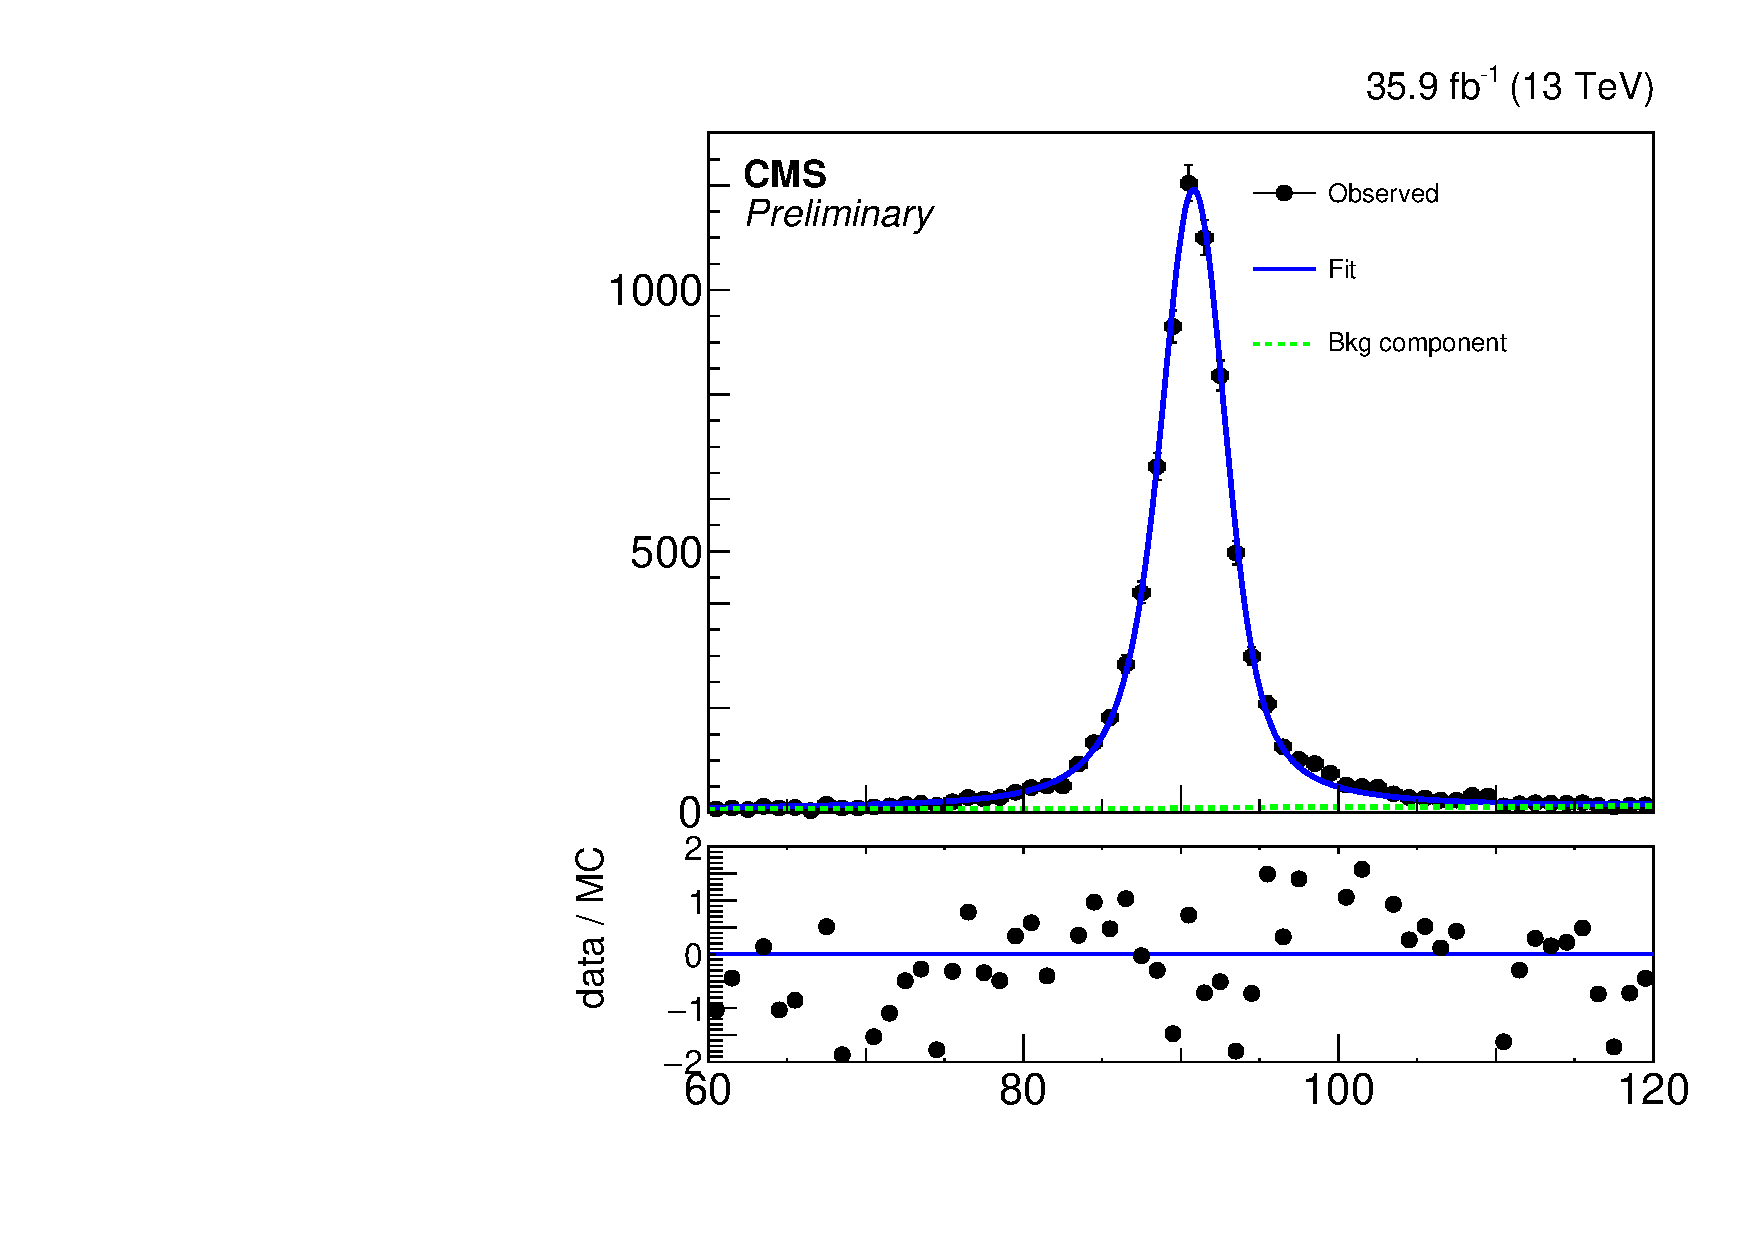
\includegraphics[width=0.48\textwidth]{Calibration/Figures/idsf/fit_data_pass_pt_175_200.pdf}
    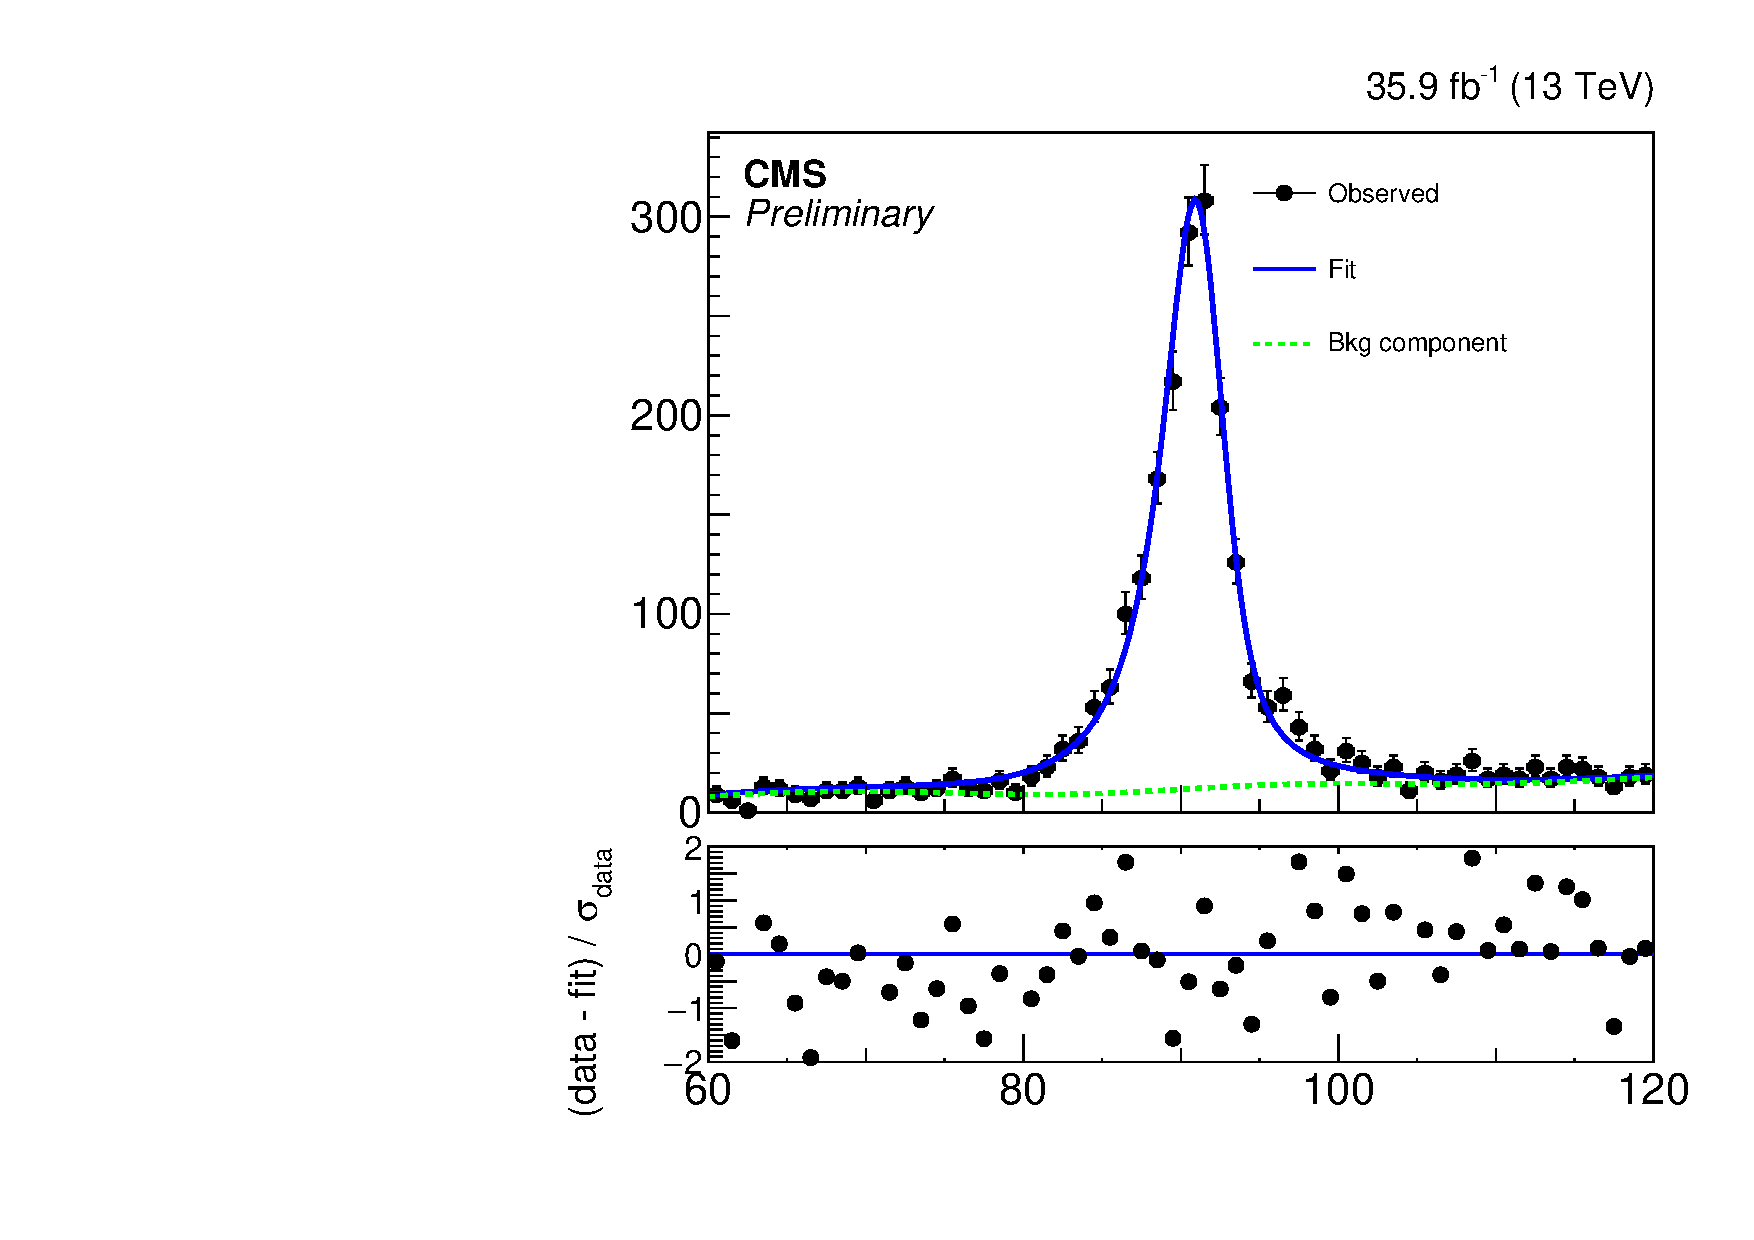
\includegraphics[width=0.48\textwidth]{Calibration/Figures/idsf/fit_data_fail_pt_175_200.pdf}
    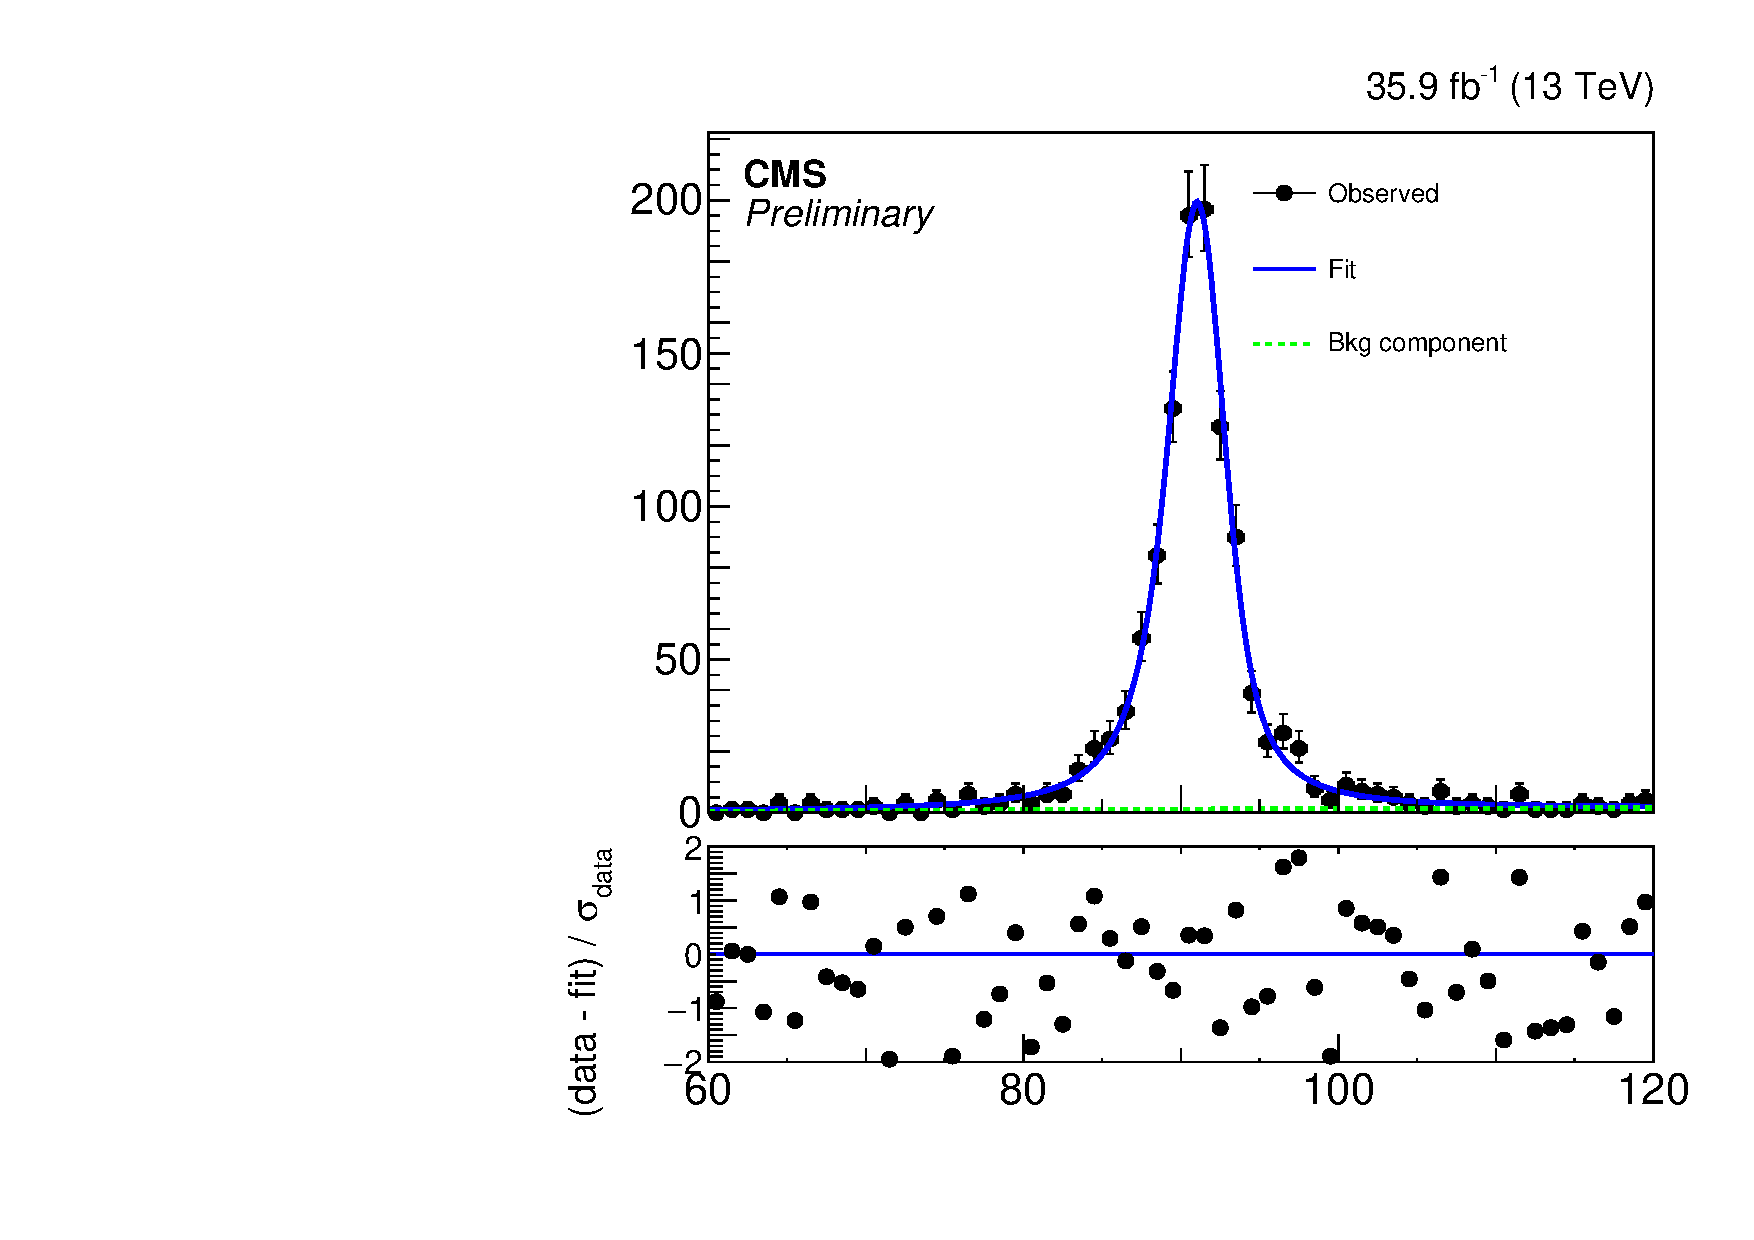
\includegraphics[width=0.48\textwidth]{Calibration/Figures/idsf/fit_data_pass_pt_300_350.pdf}
    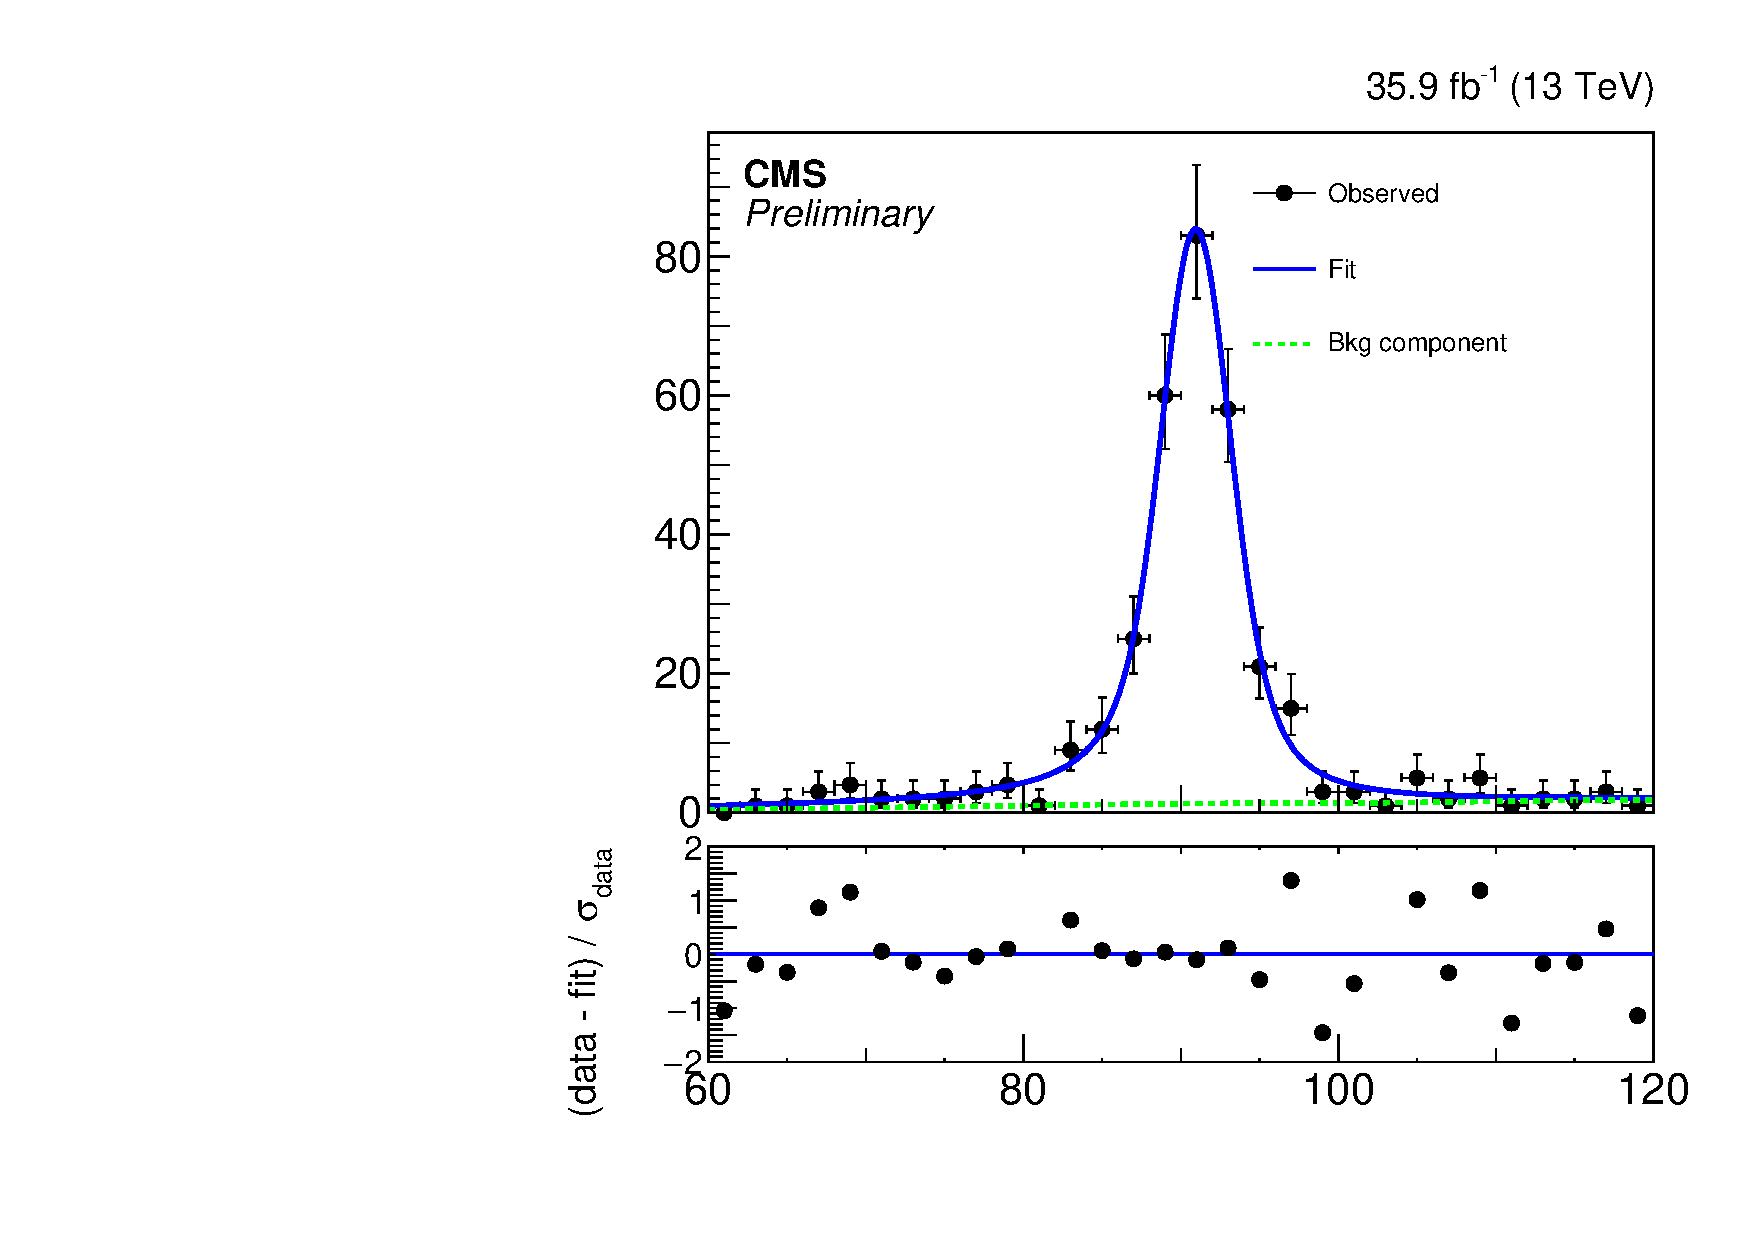
\includegraphics[width=0.48\textwidth]{Calibration/Figures/idsf/fit_data_fail_pt_300_350.pdf}
    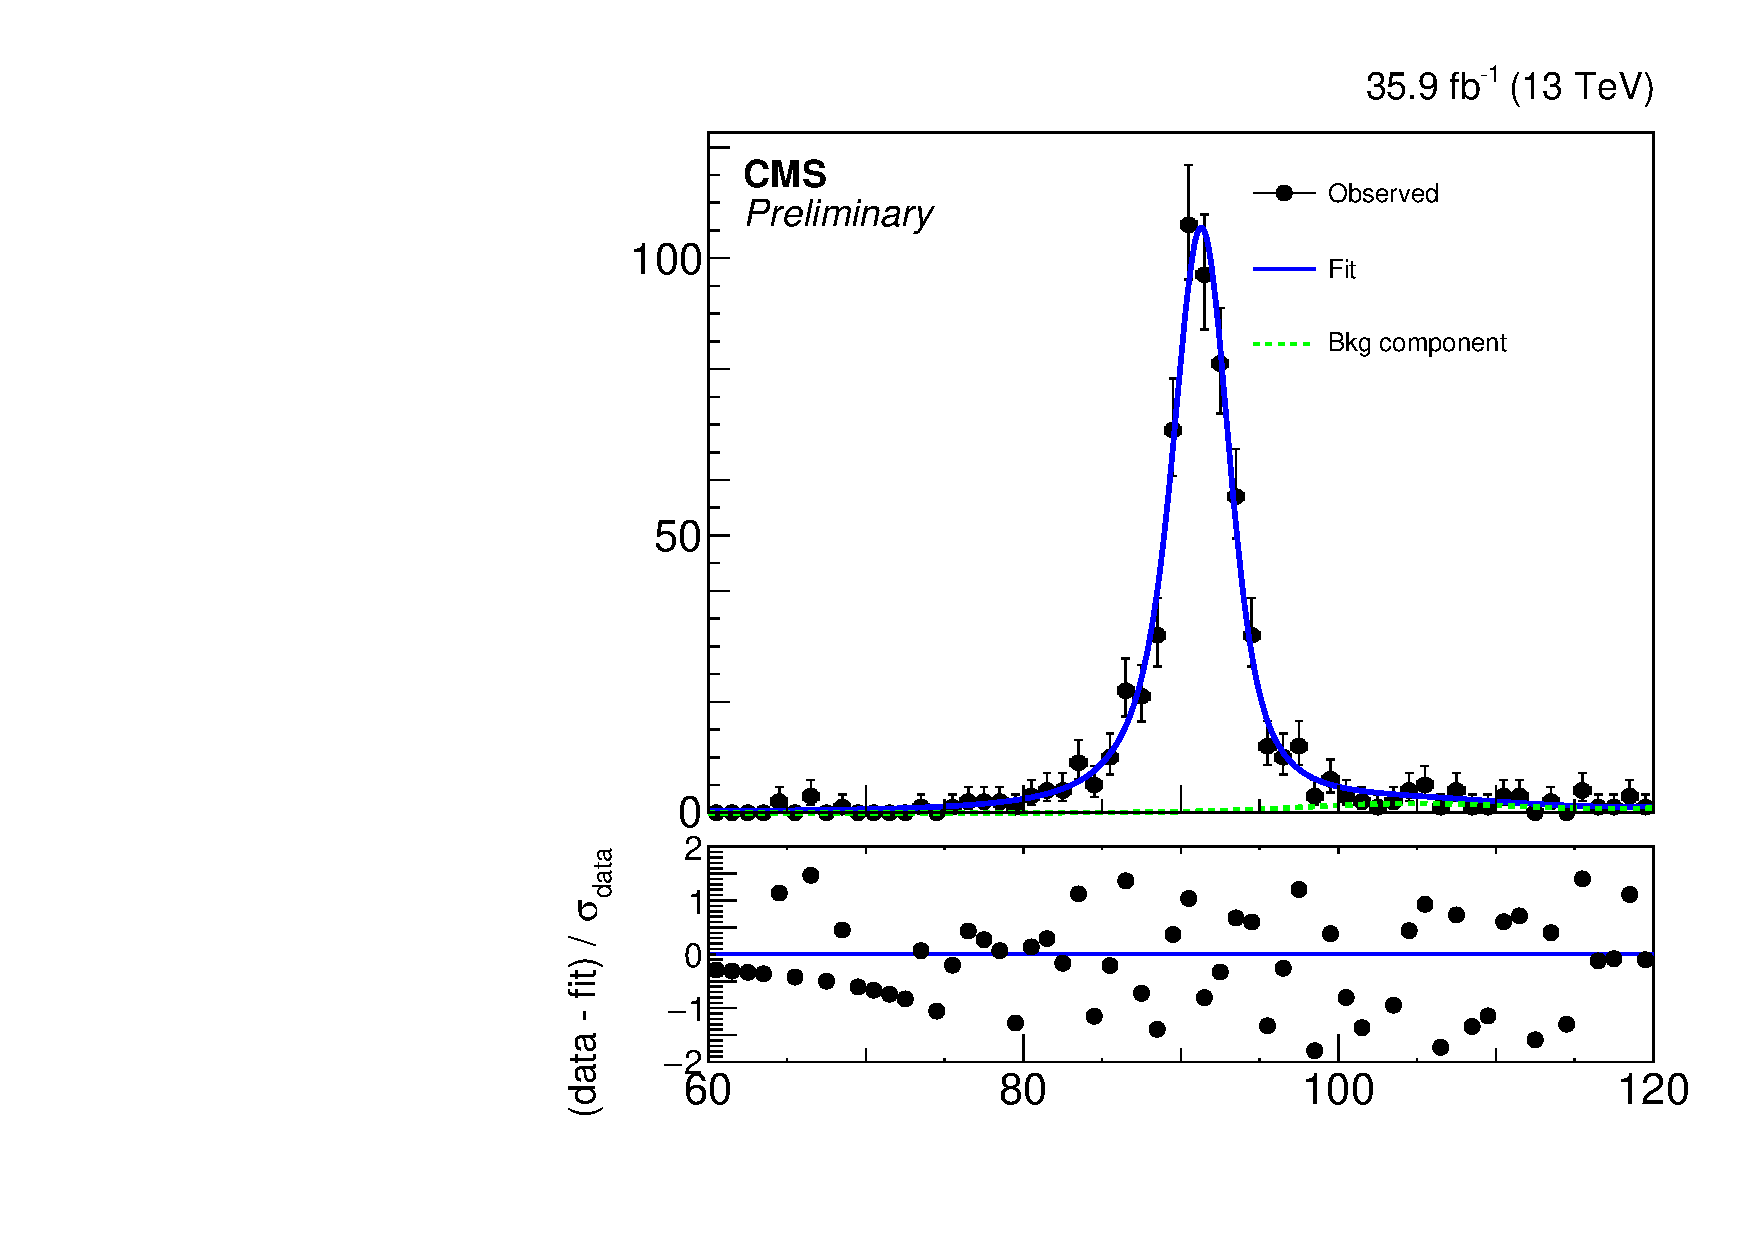
\includegraphics[width=0.48\textwidth]{Calibration/Figures/idsf/fit_data_pass_pt_400_6500.pdf}
    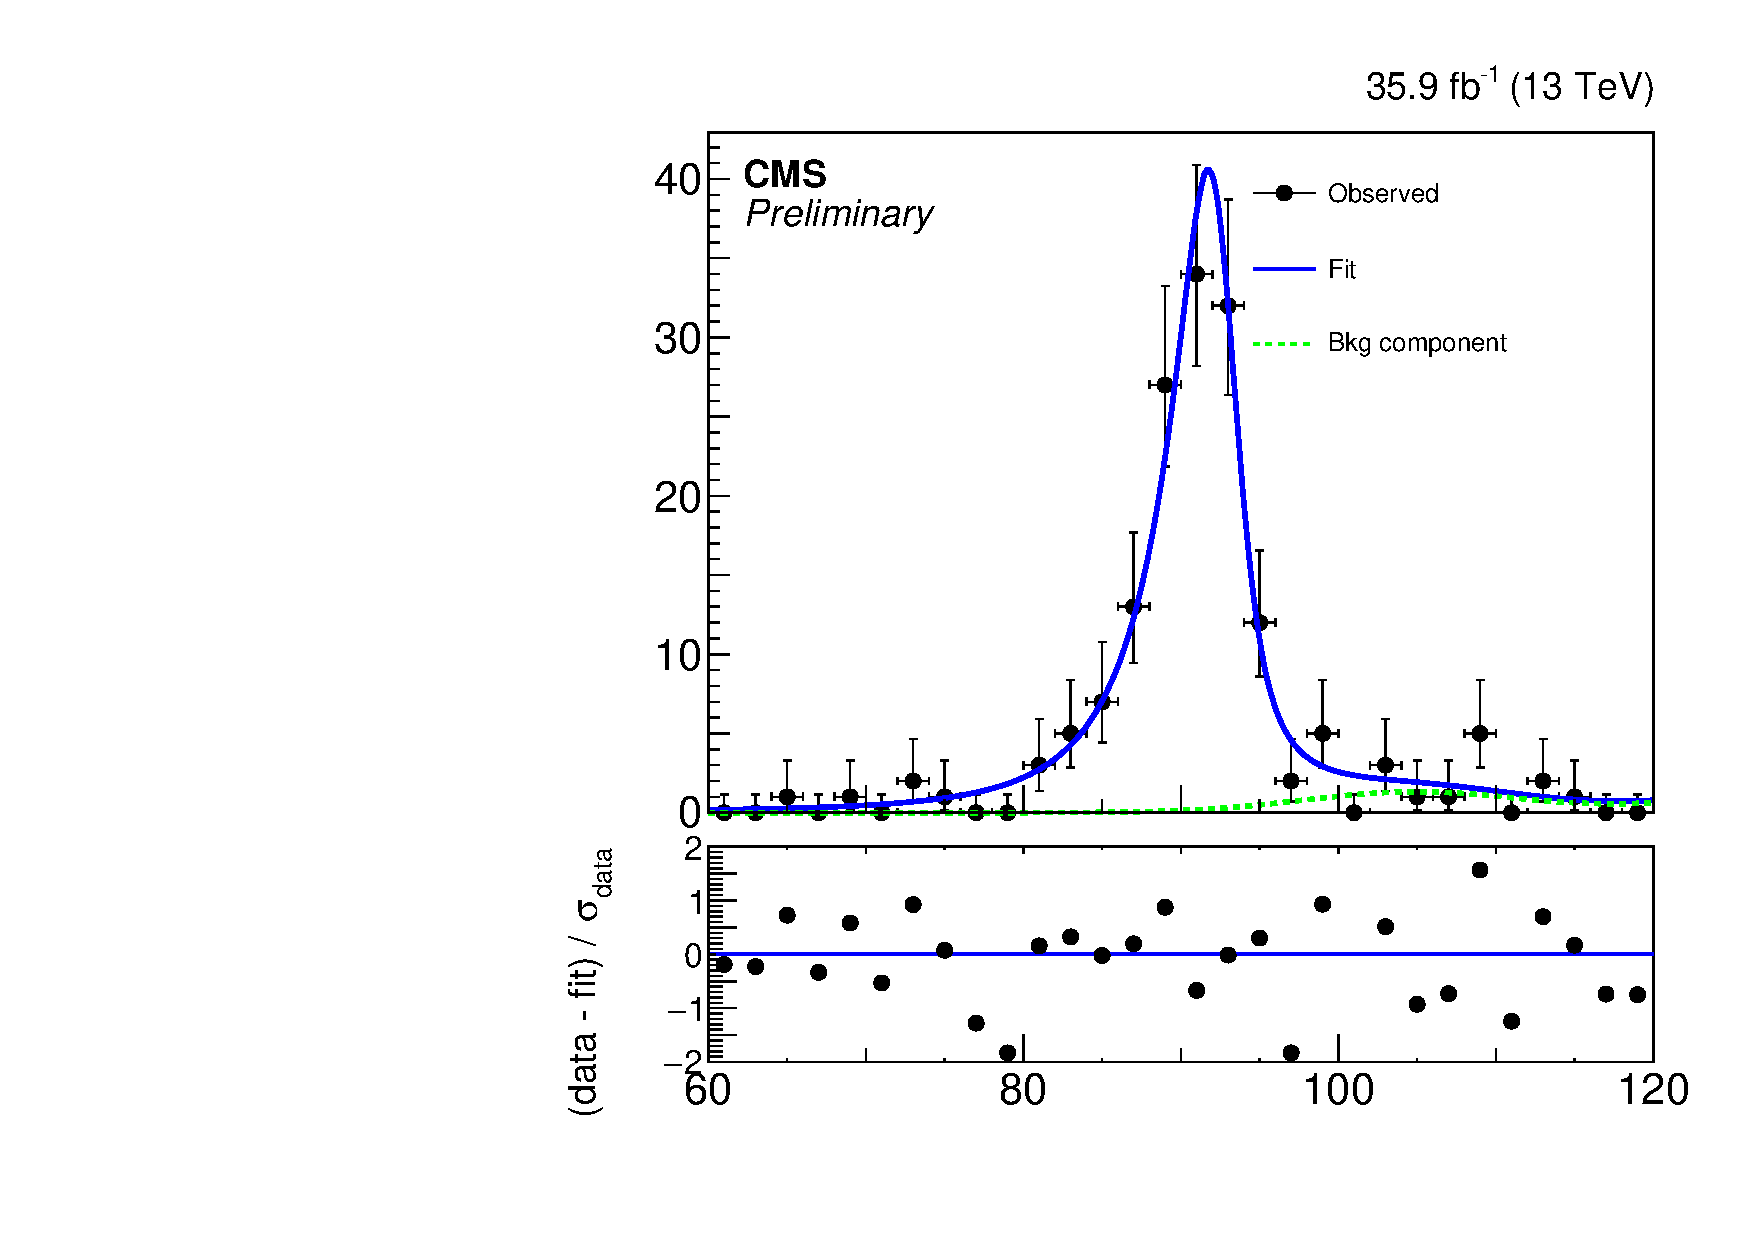
\includegraphics[width=0.48\textwidth]{Calibration/Figures/idsf/fit_data_fail_pt_400_6500.pdf}
    \caption{
      Fits to the mass distributions for pass (left) and fail (right) selections, in bins of probe \pt: 
      $175 < \pt < 200\GeV$ (top), 
      $300 < \pt < 350\GeV$ (middle), 
      $\pt > 400\GeV$ (bottom). 
      The blue solid line represents the full fit model, and the green dashed line its background component.
    }
    \label{fig:idsf_fits}
  \end{center}
\end{figure}

The statistical uncertainty of the fits is estimated by generating toy data from the nominal fit result with the same number of entries as the fit target distribution. 
The mass distribution of the toy data is then fit with the same model with the parameters floating. 
This procedure is repeated 100 times to obtain a distribution of the \Zee\ event yields, and its standard deviation is taken as the statistical uncertainty of the fit. 
Relative statistical uncertainty on the efficiency is 10\%. %%% double check this number

To estimate the effect of potential mismodeling in the fits, alternative fits varying the background and signal templates are performed first. 
In the alternative-background fit, a simple linear function is tested.
In the alternative-signal fit, no Crystal Ball convolution is performed to the signal template and the mass and width of the Breit-Wigner function are allowed to vary. 
Resulting best-fit distributions of these alternative models are then used to generate a large number of toy distributions, which are fit by the nominal model. 
The average shift of the fit result from the nominal value is then taken as the uncertainty. The relative uncertainty on the efficiency varies from 2 to 4\% depending on the probe \pt\ bin. %%% double check these numbers

The MC efficiency is taken from counting the number truth-matched electrons passing and failing the \egamma\ part of the ID from a \Zee\ sample. 
Additionally, the MC efficiency is computed using the same procedure as in data as a cross-check. The two methods are consistent within their uncertainties. 

The data efficiencies, MC efficiencies, and resulting scale factors as a function of \pt\ are shown in Figure~\ref{fig:idsf_results}. 
The scalefactors are consistent with unity within the uncertainties. 
The numerical values are given in Table~\ref{tab:idsf_results}. 
We use the bin by bin scale factor corresponding to the truth values in the analysis.

\begin{figure}[htbp]
  \begin{center}
    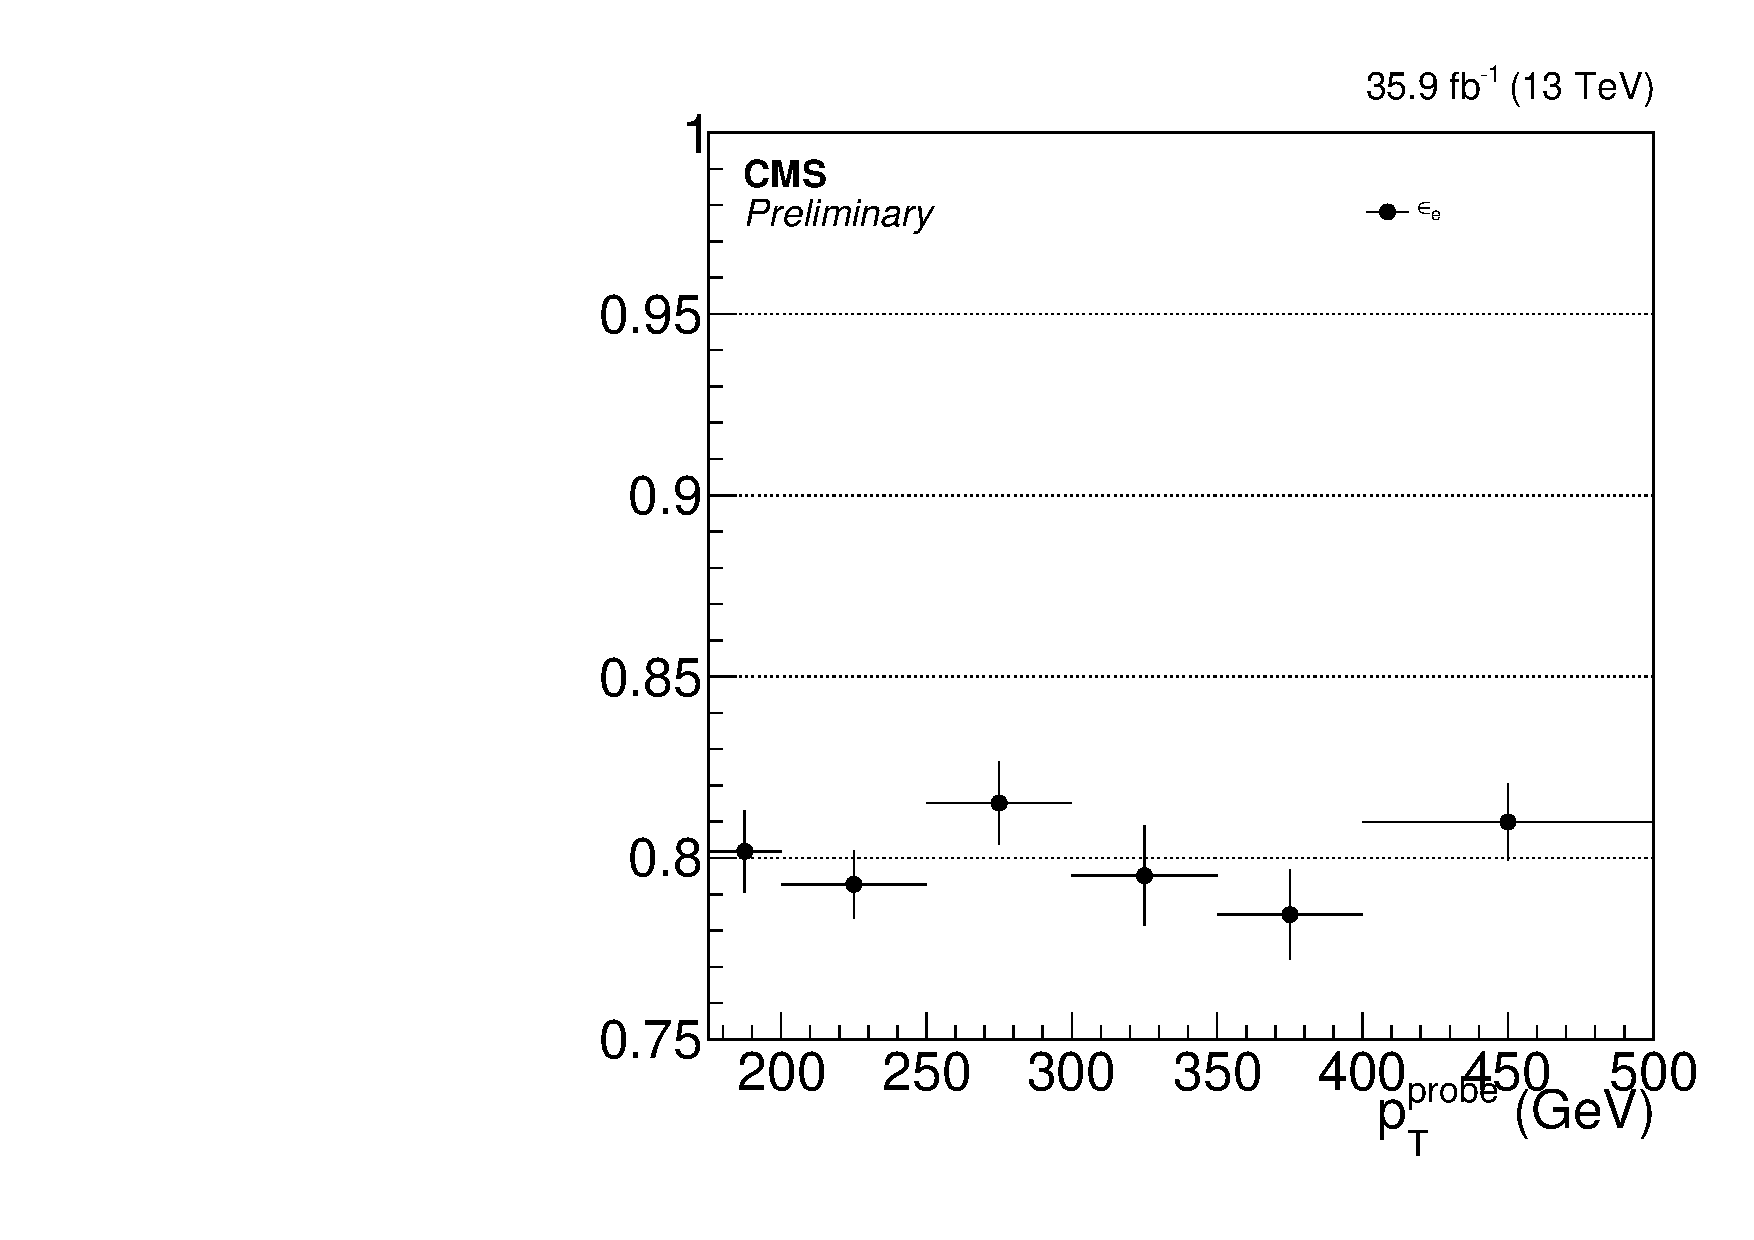
\includegraphics[width=0.48\textwidth]{Calibration/Figures/idsf/eff_data_ptalt.pdf}
    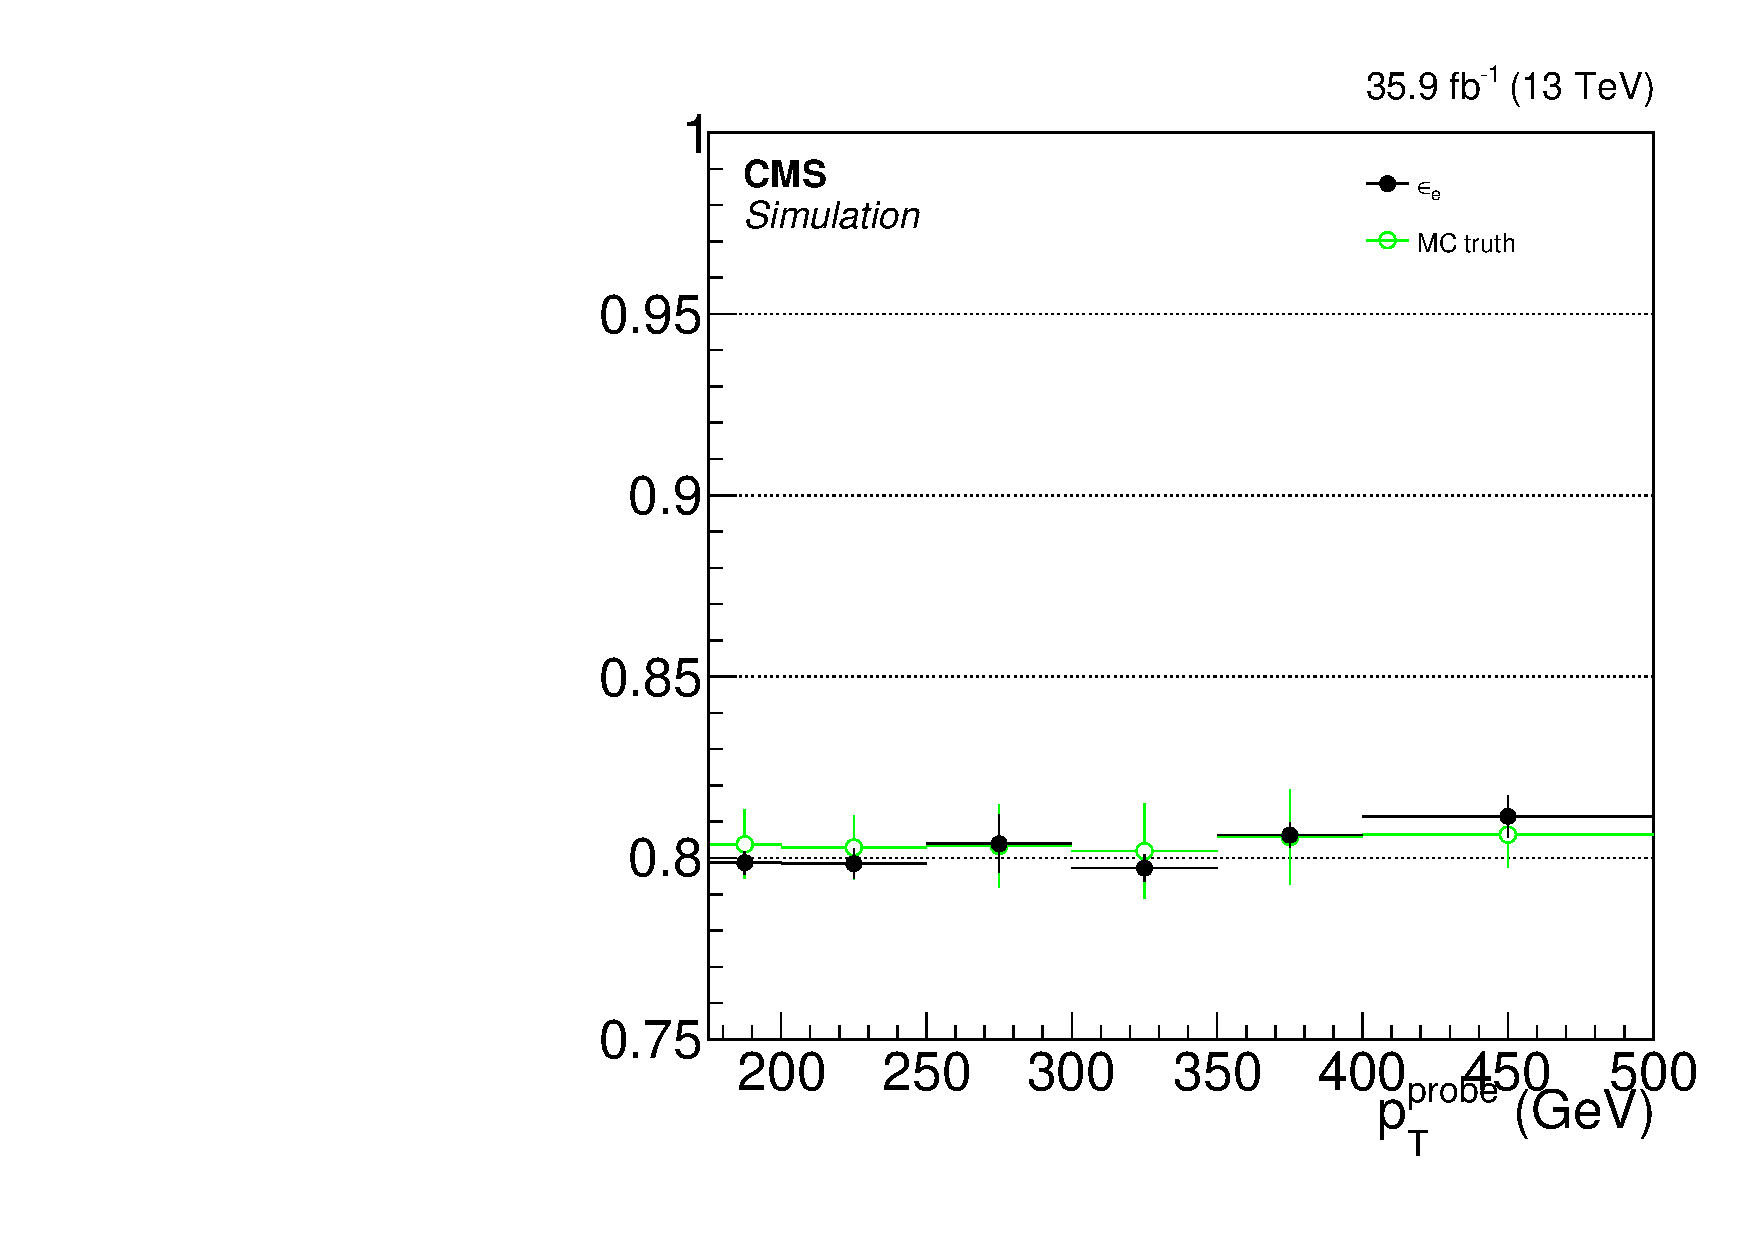
\includegraphics[width=0.48\textwidth]{Calibration/Figures/idsf/eff_mc_ptalt.pdf}
    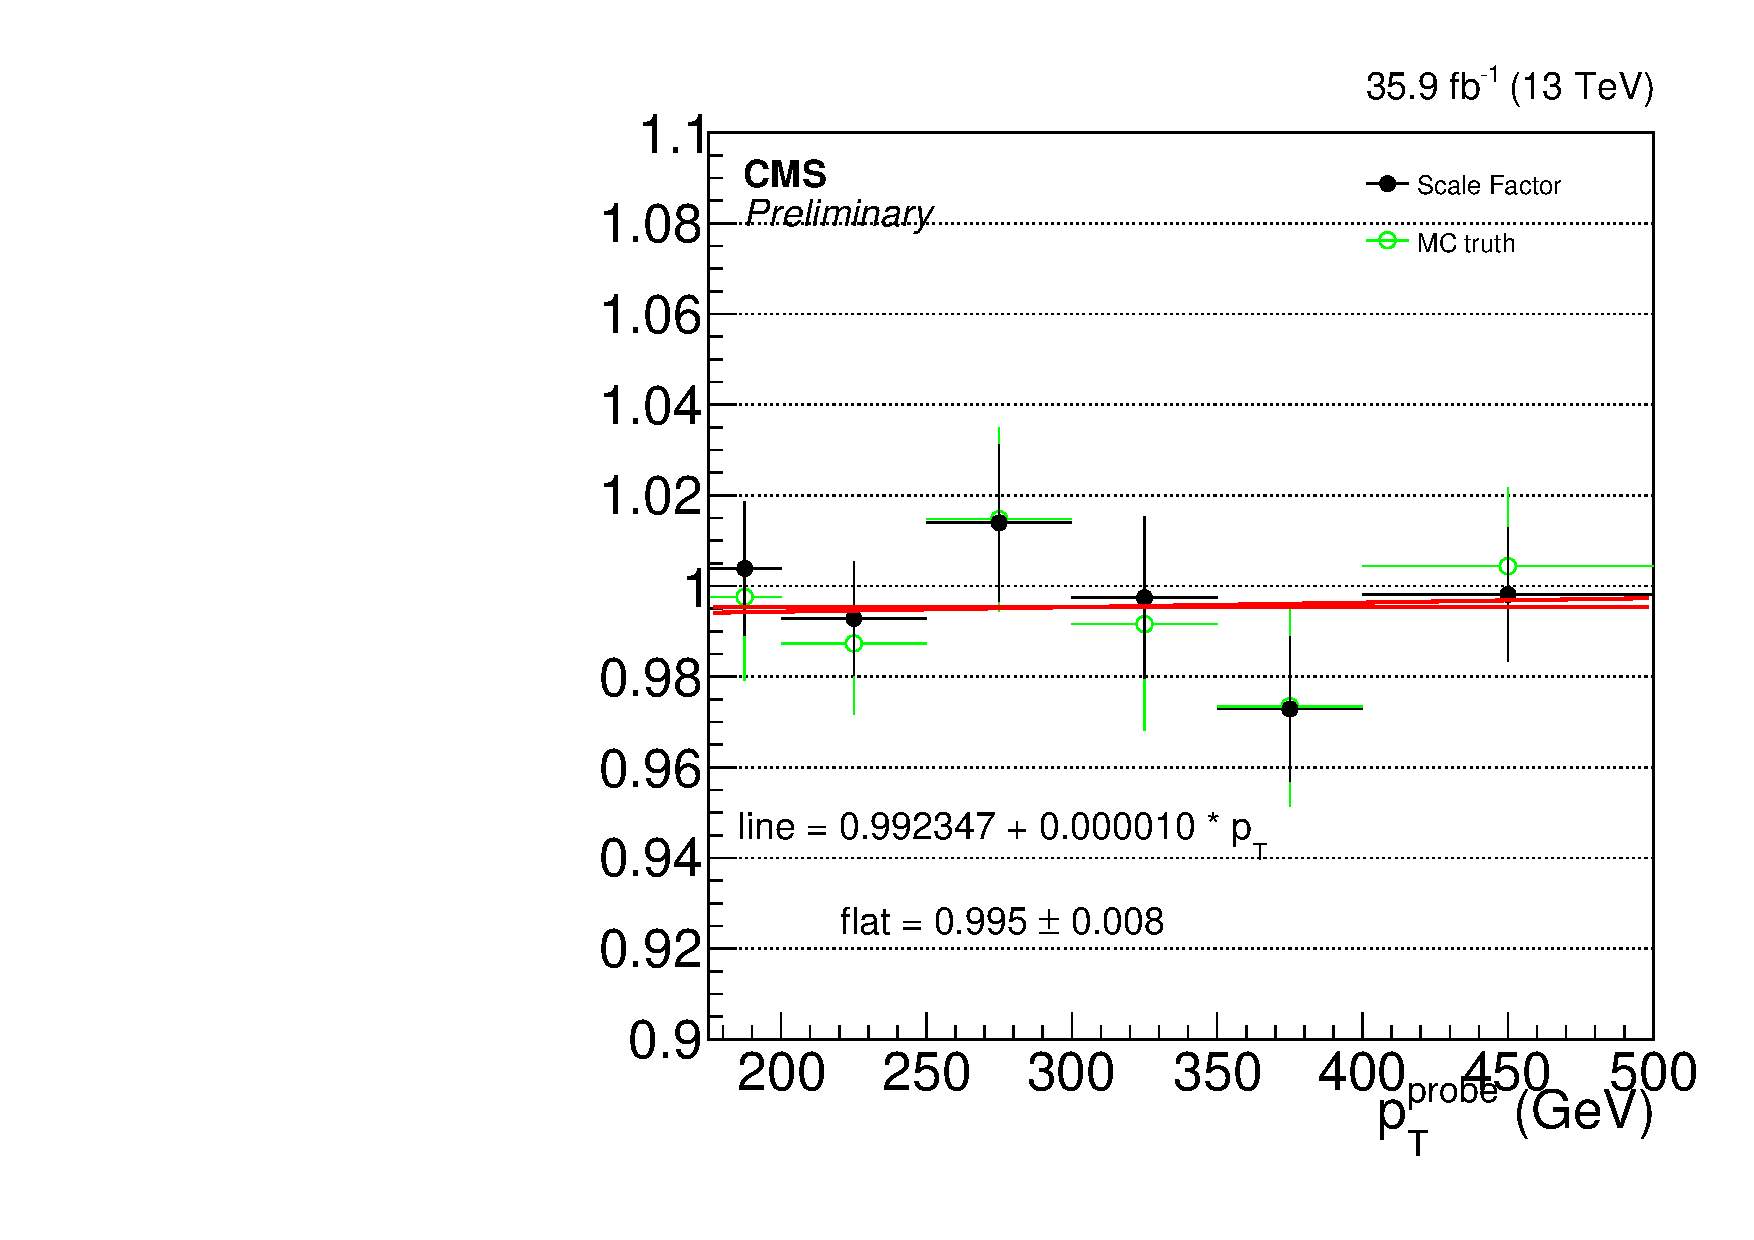
\includegraphics[width=0.48\textwidth]{Calibration/Figures/idsf/scaleFactor_ptalt.pdf}
    \caption{
      \egamma\ component of the photon identification efficiency for data (top-left) and MC (top-right) and correspending scale factor (bottom) as a function of photon \pt.
    }
    \label{fig:idsf_results}
  \end{center}
\end{figure}
 
\begin{table}[htbp]
  \begin{center}
    \caption{\egamma\ scale factors as a function of photon \pt.}
    \label{tab:idsf_results}
    \begin{tabular}{ |c|c|c| }
% \hline
% \multicolumn{3}{ |c| }{Custom ID Scale Factor for high $p_{T}$ photons} \\
\hline
 $\pt^{\mathrm{probe}}$ (GeV) & MC Fit & Truth \\\hline
 (175, 200)  & $1.014 \pm 0.008$ & $1.009 \pm 0.016$ \\
 (200, 250)  & $1.003 \pm 0.008$ & $0.999 \pm 0.014$ \\
 (250, 300)  & $1.014 \pm 0.010$ & $1.016 \pm 0.019$ \\
 (300, 350)  & $1.002 \pm 0.014$ & $0.997 \pm 0.022$ \\
 (350, 400)  & $0.986 \pm 0.012$ & $0.987 \pm 0.022$ \\
 (400, 6500)  & $0.988 \pm 0.011$ & $0.999 \pm 0.016$ \\
\hline
\end{tabular}

  \end{center}
\end{table}

\subsection{\Pgg-specific ID Efficiency}
\label{subsec:pvsf}

To measure the efficiency of the \Pgg-specific component of the photon ID, we use a \sieie\ template fit to extract the number of true photons from a pool of photon objects passing the \egamma\ ID.

The measurement is performed over a EM object+jet control sample where we require one jet passing with $\pt > 100\GeV$ and $|\eta| < 2.5$ which passes the loose jet ID. 
The EM object passes the \egamma\ ID with the execption of the following relaxed cuts: 
\begin{itemize}
\item $\sieie < 0.015$
\item $\ICH < 11.0\GeV$ .
\end{itemize}
Additionally, we apply a $\met < 60\GeV$ cut to make this region orthogonal to the signal region of the analysis.

We then fit the \sieie\ distribution of the EM object with a template describing the \sieie\ shape of true photons and another describing the hadronic background. 
The real photon template is taken from \gj\ MC requiring the photon to pass the \egamma\ ID except for the \sieie\ requirement.
The fake photon template is taken from the same data control sample, requiring $5\GeV < \ICH
< 7\GeV$. 
The integral of the post-fit real photon template below $\sieie = 0.0104$ is the number of true photons in the target sample.

The fit is performed once for all EM objects and then once for EM objects passing the \Pgg-specific ID criteria. 
The ratio of the numbers of true photons obtained in the two fits is the efficiency.

The \sieie\ template fit method in its simplest form fits the observed distribution with the following fit function:
\begin{align}
  P(f;\sieie) = f \cdot h_{s}(\sieie) + (1 - f) \times h_{b}(\sieie),
\end{align}
where $h_{s}$ is the signal template, $h_{b}$ is the background template, and $f$ is the fraction of true photons in the target sample. 
Both the target template and the fit function are normalized to unity, removing the number of photon candidates in the target sample $N$ as a fit parameter and leaving $f$ as the only free parameter.

However, the hadronic background template, taken from the data control sample, has contributions from real photons. 
The amount of this ``photon contamination'' depends on the sideband choice, but is finite even for a sideband with very large \ICH. 
As described below, we perform additional fits with the background templates from alternative sidebands $3.5\GeV < \ICH < 5\GeV$ (``near'') and $7.5\GeV < \ICH < 9\GeV$ (``far'') to assess the systematic uncertainty. 
The photon contamination of the nominal and far sideband is 10-15\%, and in the near sideband, it can go up to approximately 20\% (see Figure~\ref{fig:impurity-signal-contamination}).

\begin{figure}[htbp]
  \centering
  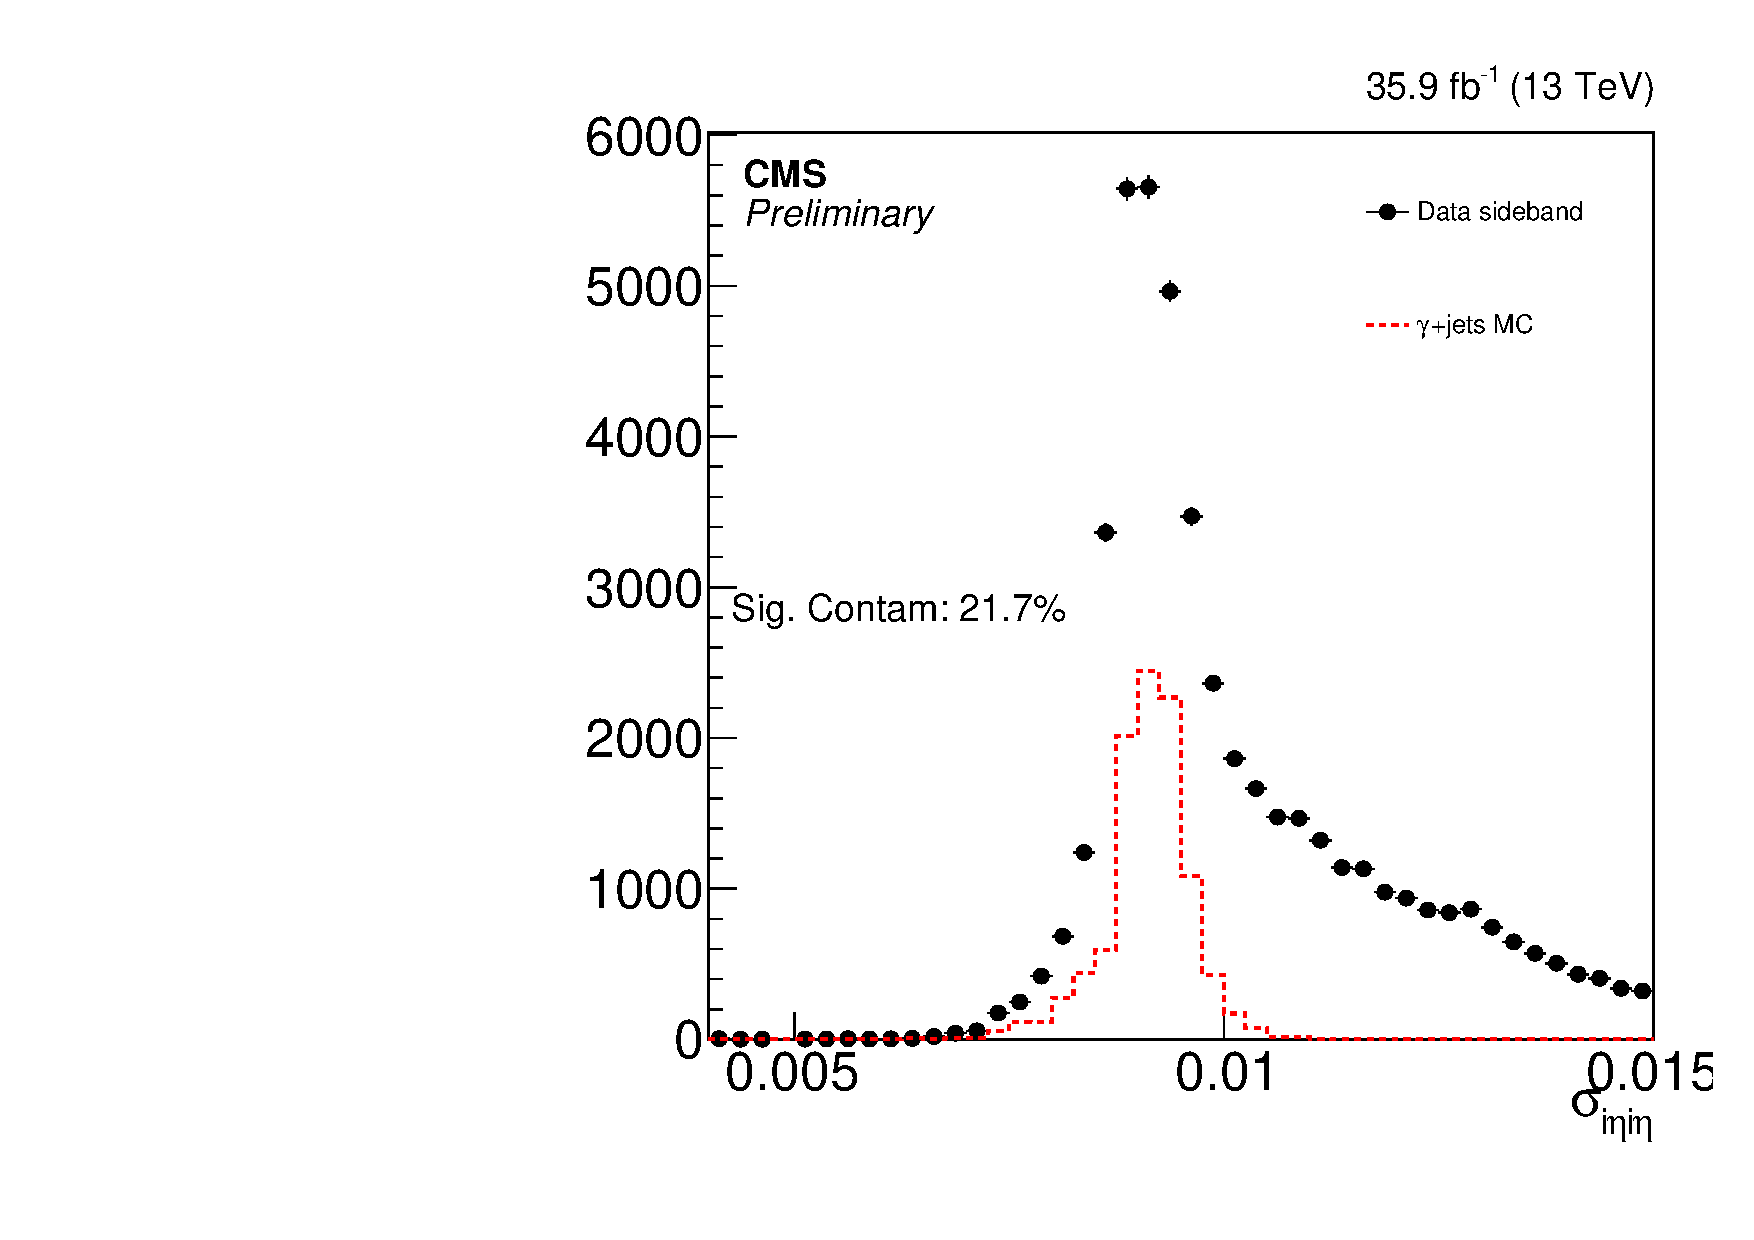
\includegraphics[width=0.45\textwidth]{Calibration/Figures/pvsf/sbcontam_near.pdf}
  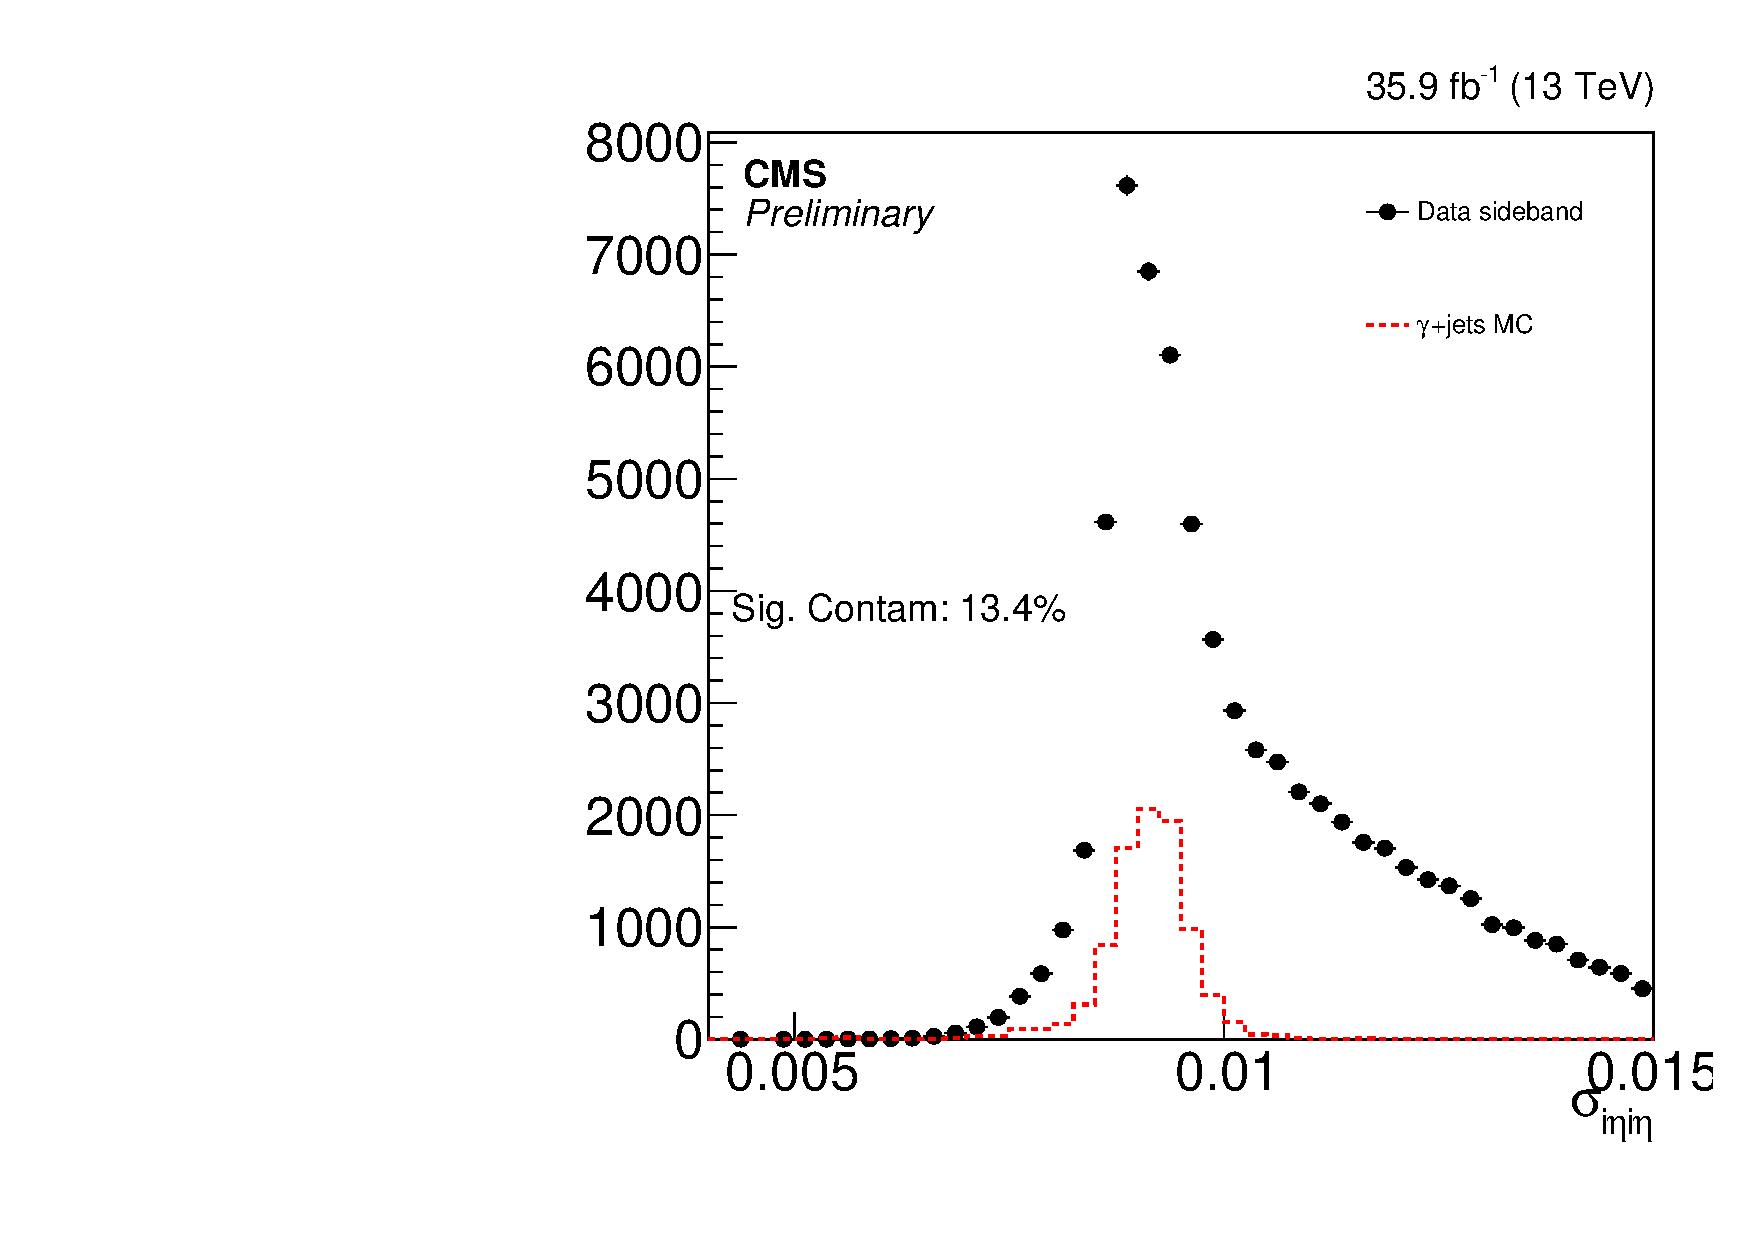
\includegraphics[width=0.45\textwidth]{Calibration/Figures/pvsf/sbcontam_nominal.pdf}
  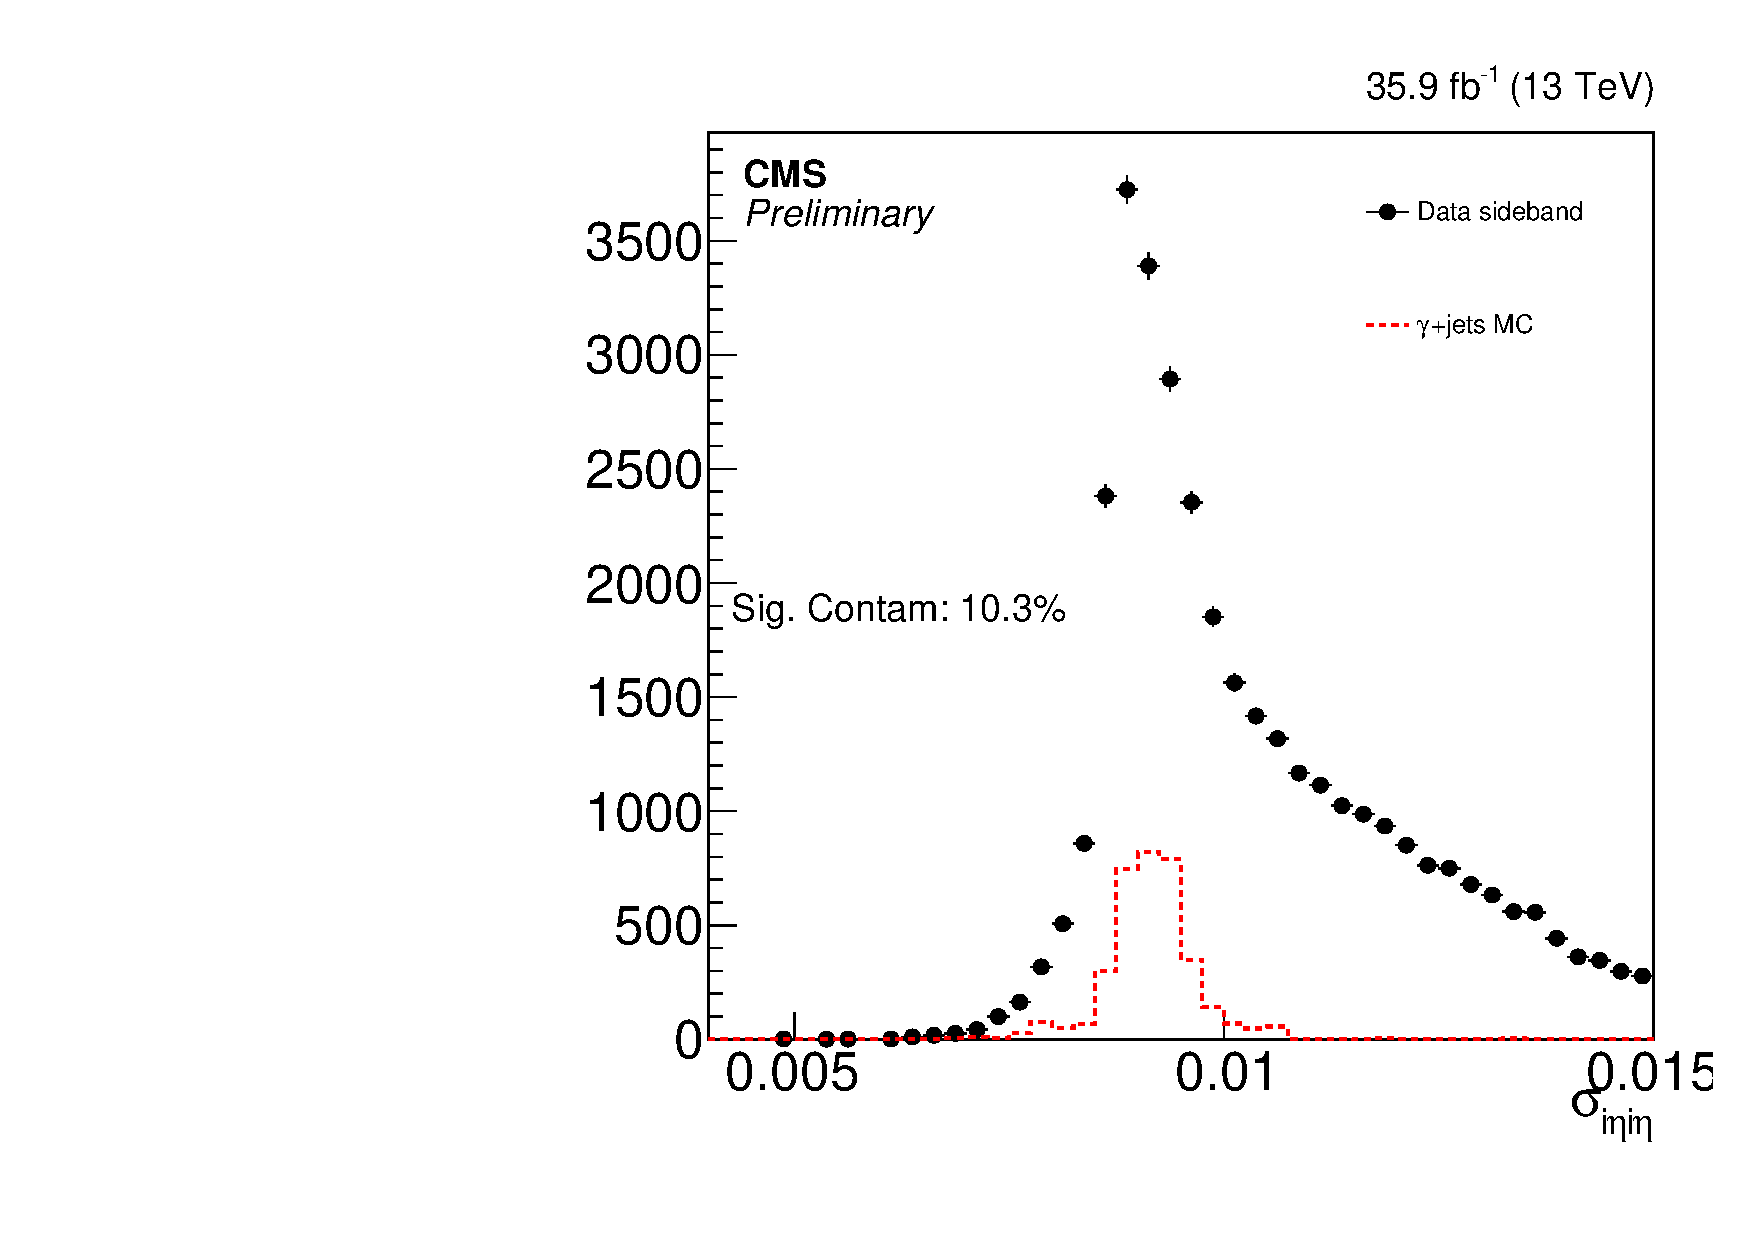
\includegraphics[width=0.45\textwidth]{Calibration/Figures/pvsf/sbcontam_far.pdf}
  \caption{
    Signal contamination in the [3.5,5.0] (left), [5.0,7.5] (middle), and [7.5,9.0] (right) isolation sidebands.
  }
  \label{fig:impurity-signal-contamination}
\end{figure}

To remove the photon contamination from the background templates, we modify the method and create a new background template $h_{b}^{\text{sub}}$ from the original background template $h_{b}$ by subtracting the true photon shape in the sideband $h_{S^{'}}$. 
After normalization to unity, we obtain the expression
\begin{align}
  h_{b}^{\text{sub}}(\sieie) = \frac{h_{b}(\sieie) - S'/B \cdot h_{s'}(\sieie)}{1 - S'/B},
\end{align}
where $B$ is the number of photon candidates in the sideband and $S'$ is the number of true photons in the sideband.

To determine $S'$, we start with the number of true photons in the target sample, $f \cdot N$. 
We then scale this by the ratio of the relative fractions of true MC photons in the \ICH\ sideband $r_{\text{sb}}$ and in the signal region $r_{\text{sig}}$, giving us the expression
\begin{align}
  S' = f \cdot \frac{r_{\text{sb}}}{r_{\text{sig}}} \cdot N .
\end{align}

Going back to our original fit function and replacing $h_{b}$ with $h_{b}^{\text{sub}}$ gives us
\begin{align}
  P(f;\sieie) = f \cdot h_{s}(\sieie) + (1 - f) \times \frac{h_{b}(\sieie) - S'(f)/B \cdot h_{s'}(\sieie)}{1 - S'(f)/B},
\end{align}
which converges to the original fit function if $S' = 0$, \ie, if there is no photon contamination in the sideband. 
Note that $f$ is still the only free parameter for this new function as $S'$ only depends on $f$ and $r_{\text{sb}} / r_{\text{sig}}$ is set constant in the fit (see discussion of systematics for more detail).


There are four main sources of systematic uncertainty for this measurement. 
The first comes from the sideband choice, as the relative rates of different types of fake photons varies with \ICH. 
The second comes from the true photon \ICH\ shape, as this is used to determine the normalization of true photons in the sideband. 
Currently, this shape is taken from MC and thus there is the potential to mismodel the effects of the underlying event and pile-up. 
The third comes from the true photon \sieie distribution. 
As we take this from MC as well, we can mismodel the signal template shape. 
Finally, at high \pt, we suffer from low yields in our \ICH\ sidebands, which can lead to
fluctutations that unduly influence the fit.

The uncertainty due to sideband choice is simply the larger of the differences of the purities measured using the near and far sidebands versus the nominal sideband. 
Figure~\ref{fig:impurity-sideband} shows fits using the three sidebands for the [400,$\infty$) \pt\ bin.

\begin{figure}[htbp]
  \centering
  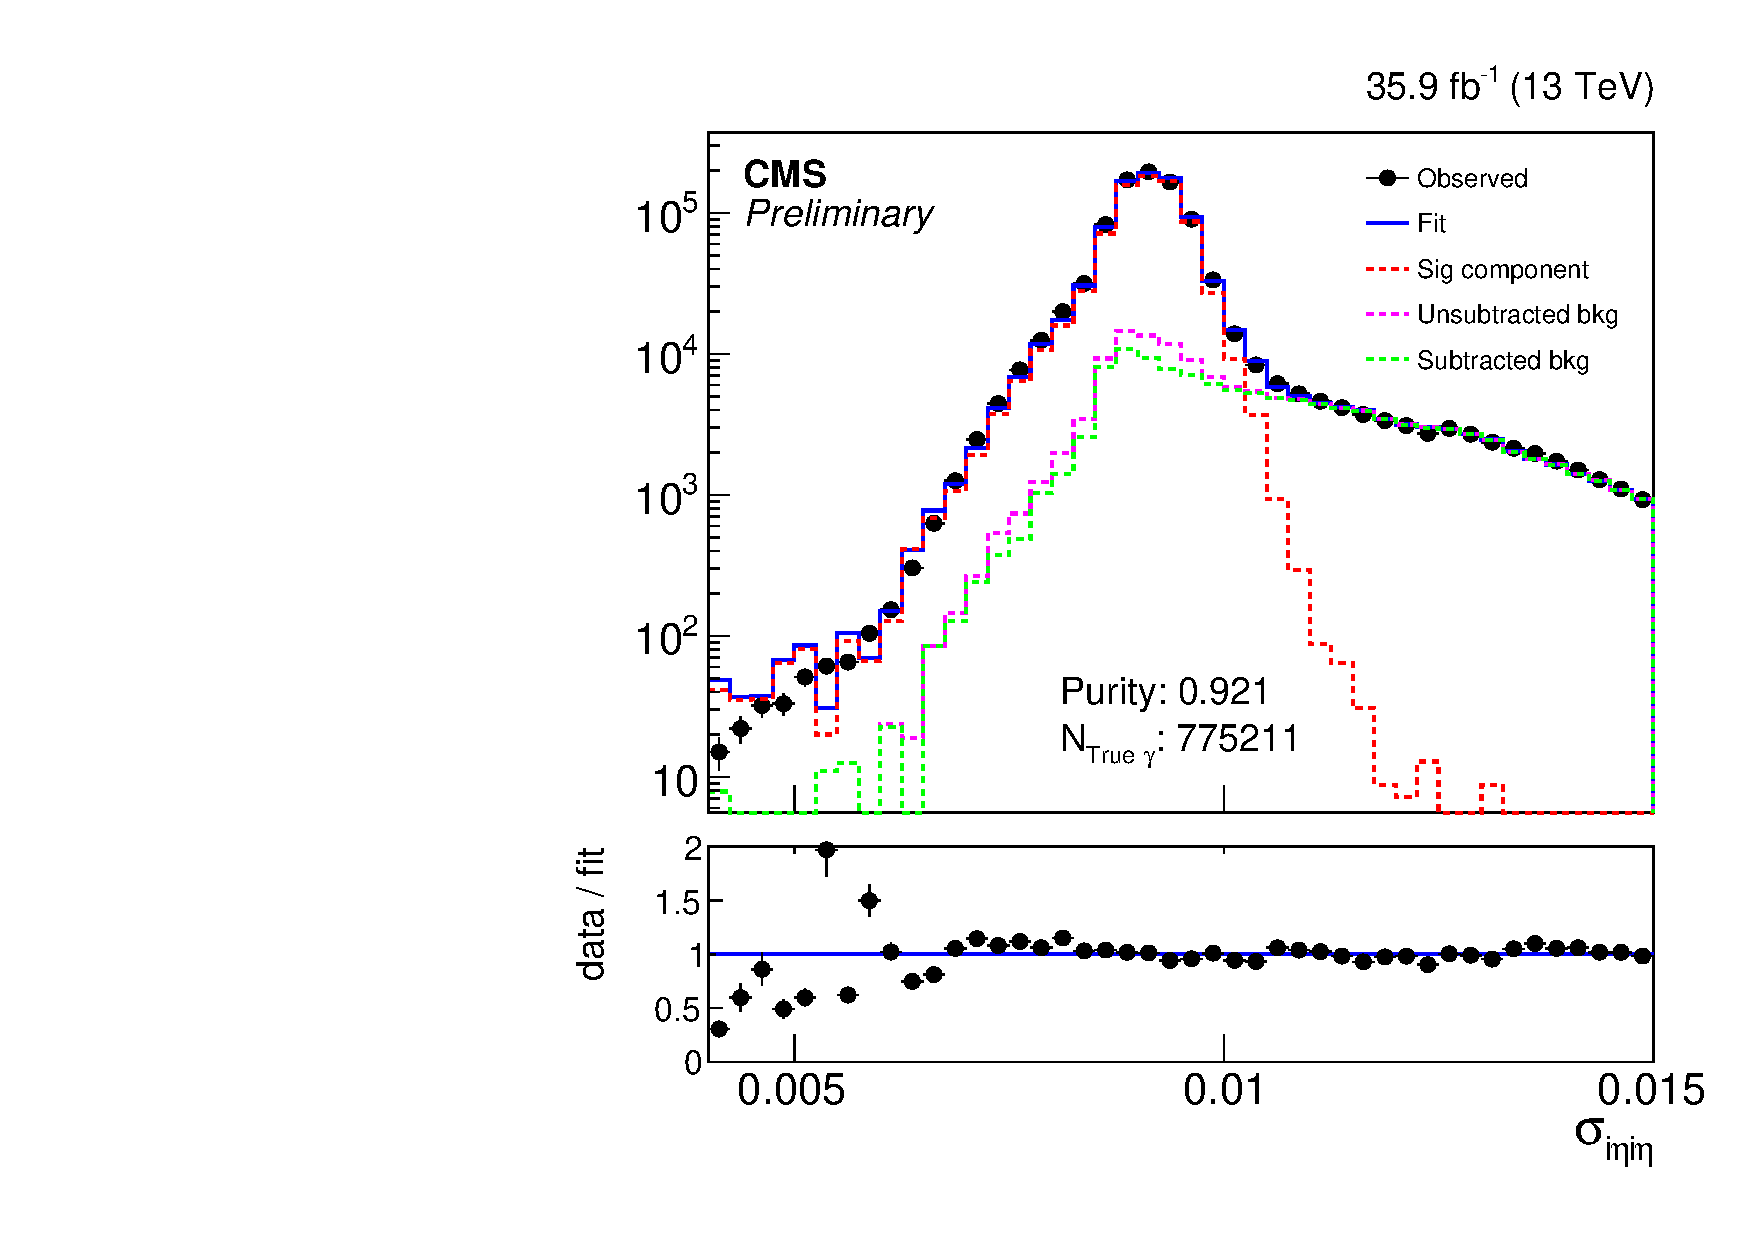
\includegraphics[width=0.45\textwidth]{Calibration/Figures/pvsf/ssfit_175_medium_near_logy.pdf}
  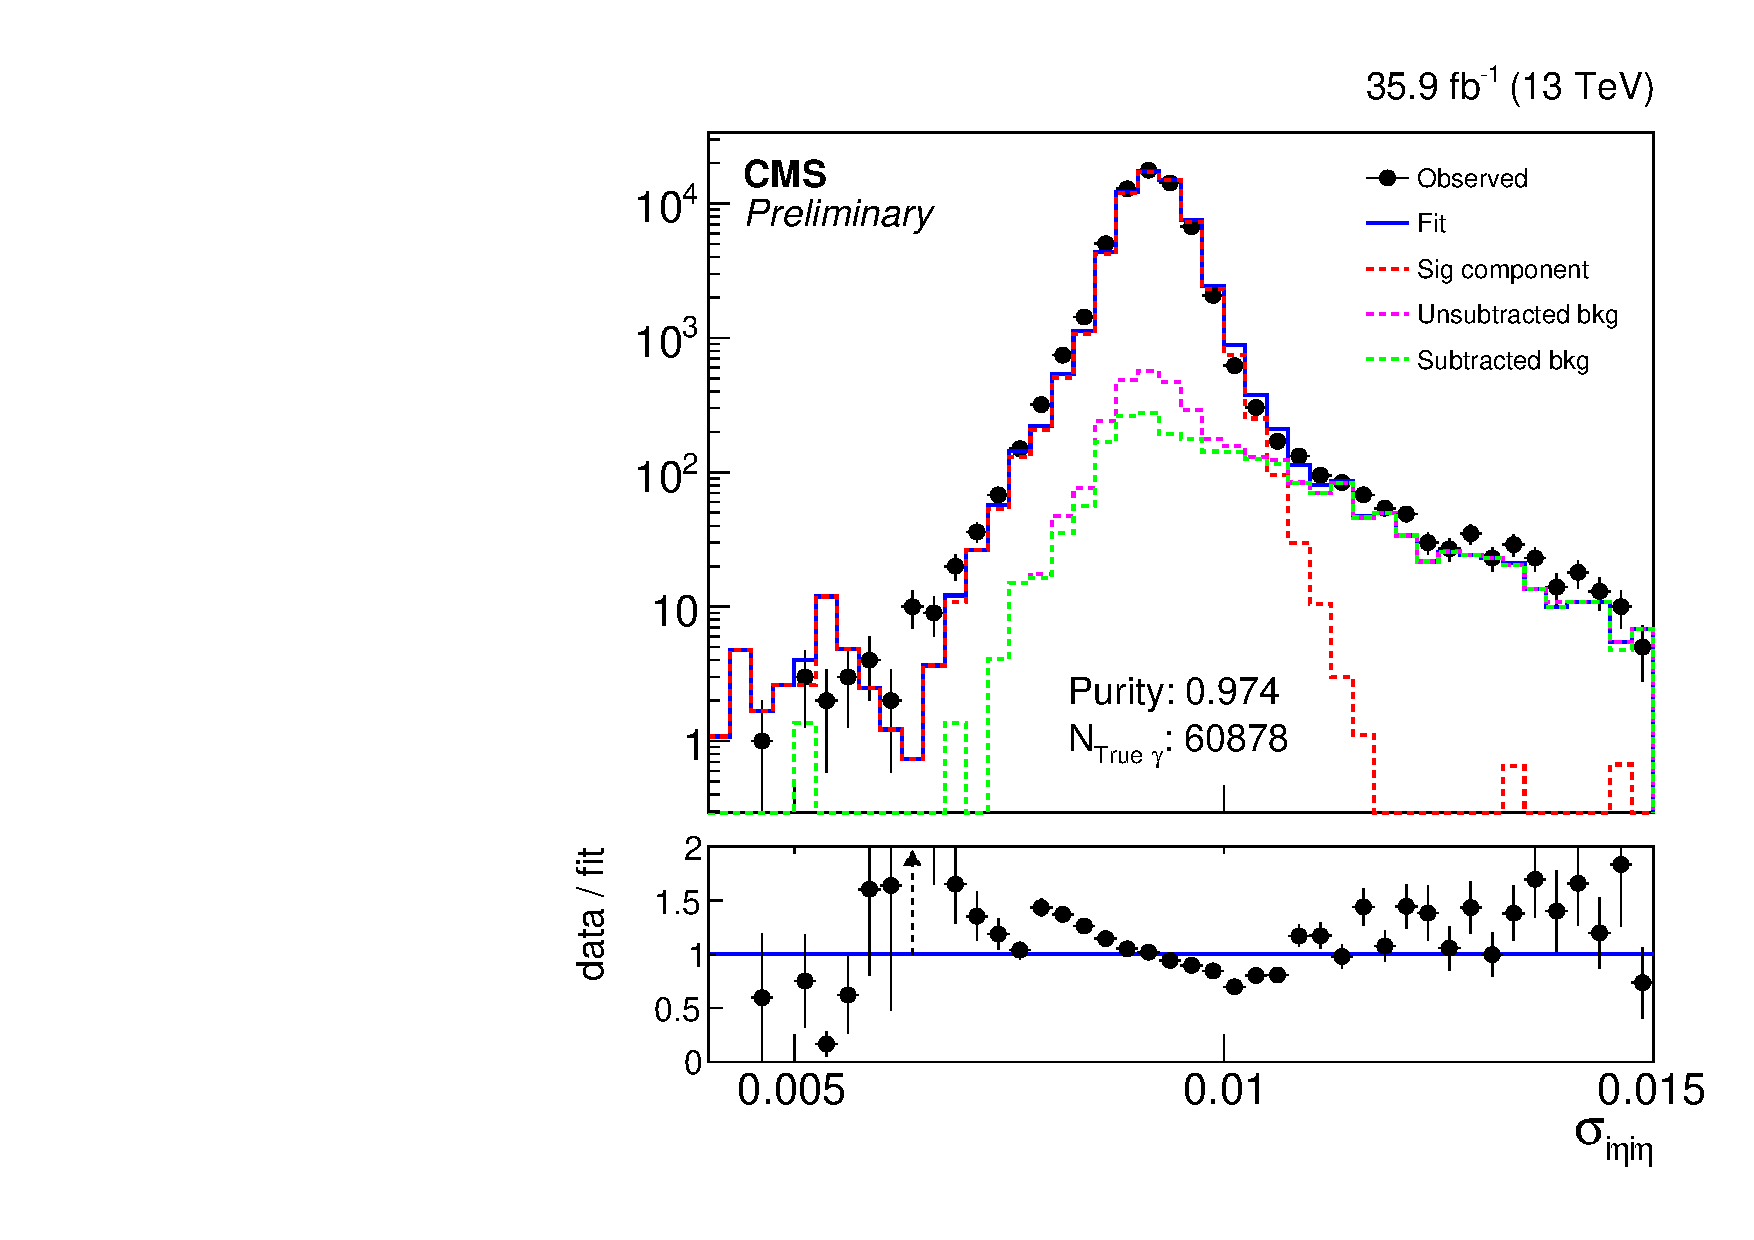
\includegraphics[width=0.45\textwidth]{Calibration/Figures/pvsf/ssfit_400_medium_near_logy.pdf}
  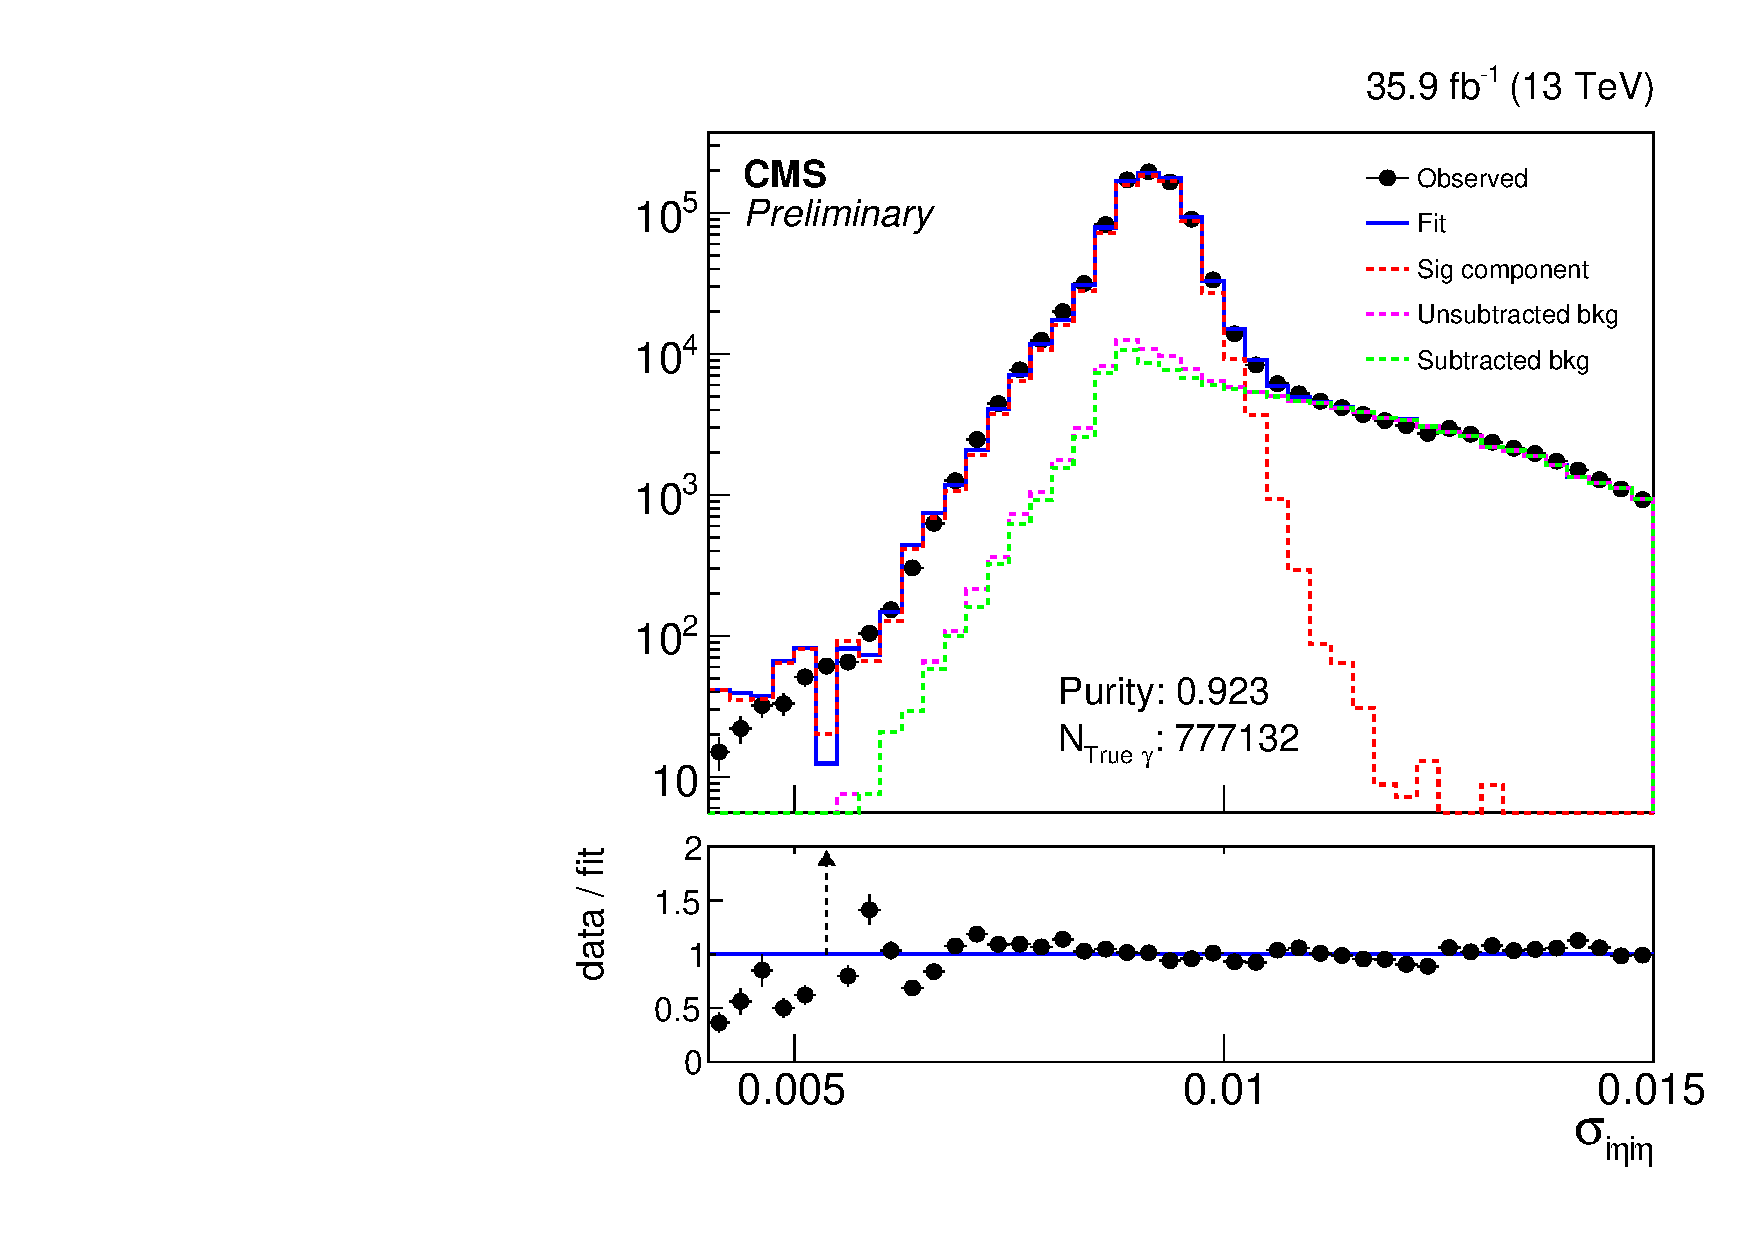
\includegraphics[width=0.45\textwidth]{Calibration/Figures/pvsf/ssfit_175_medium_nominal_logy.pdf}
  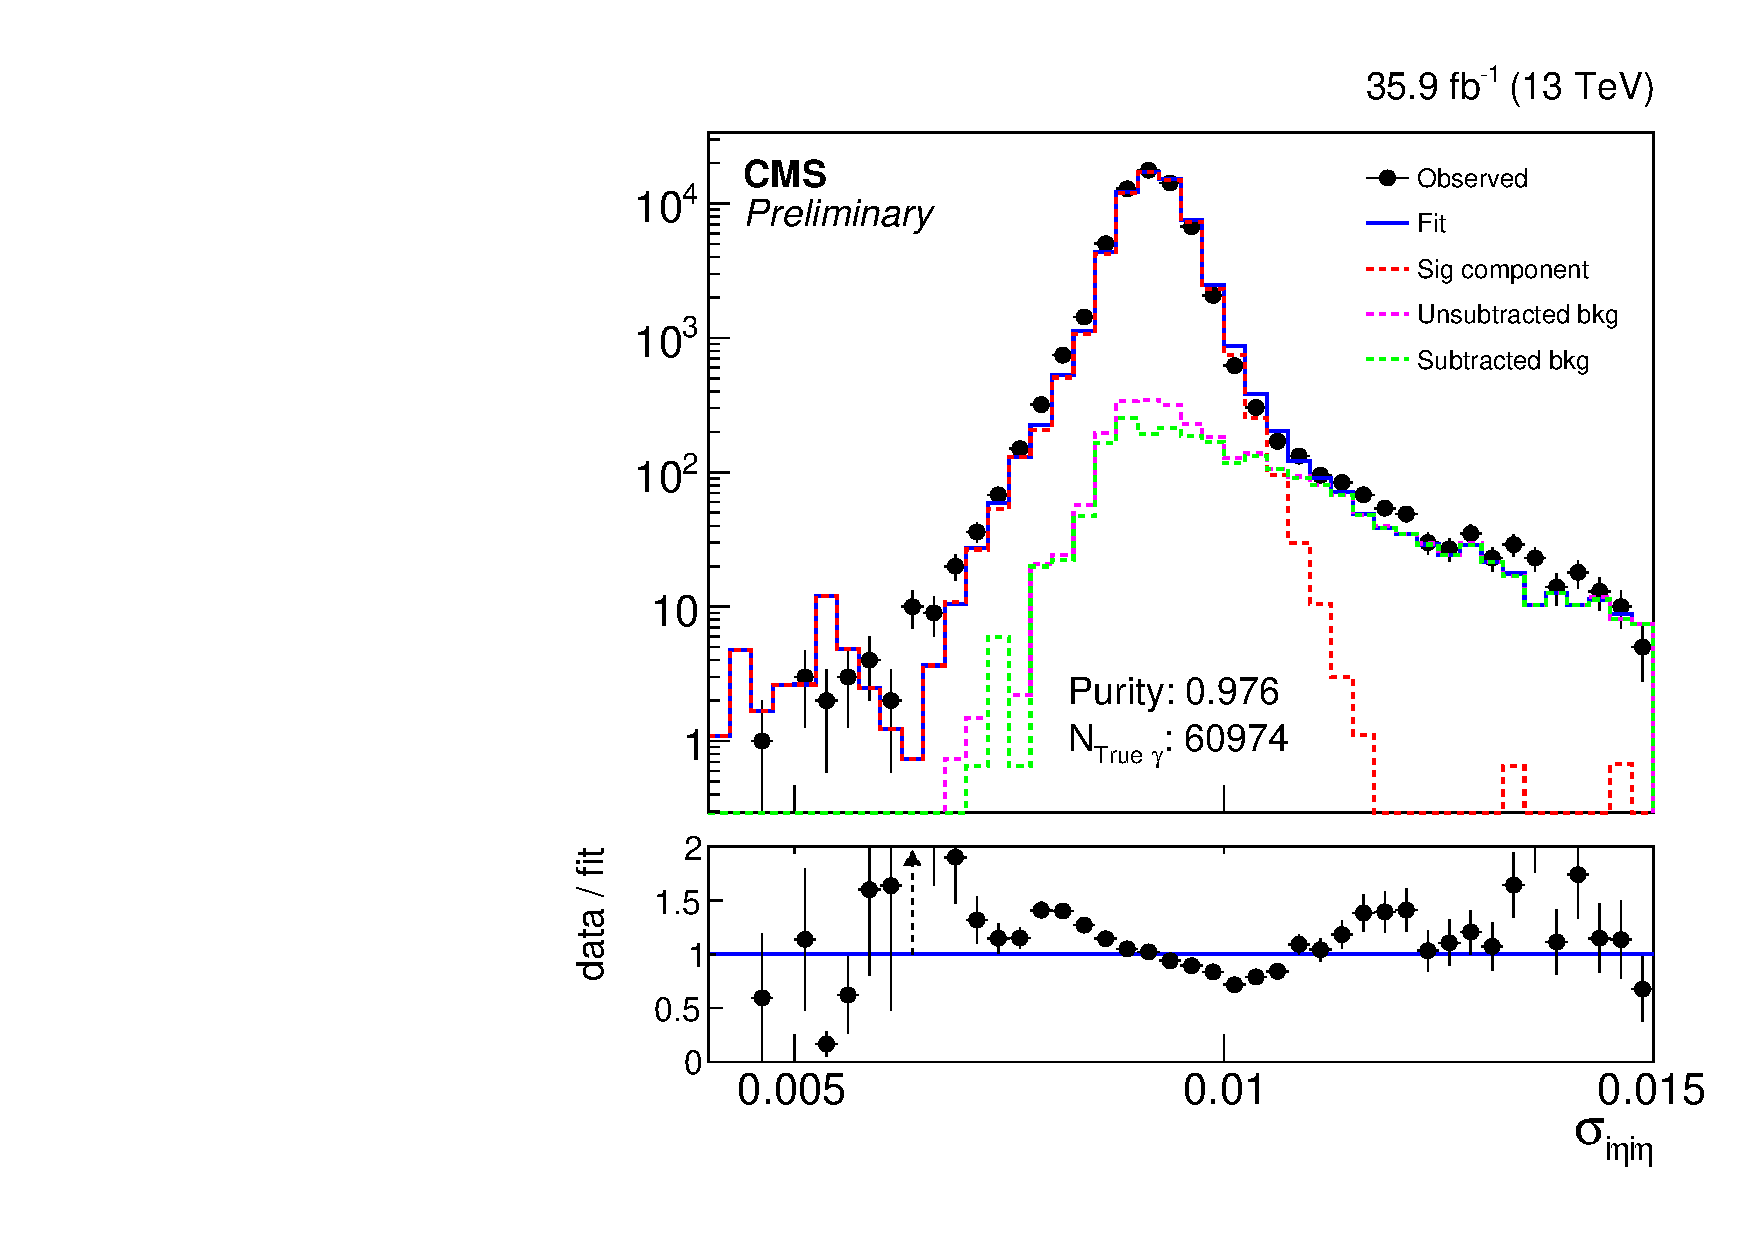
\includegraphics[width=0.45\textwidth]{Calibration/Figures/pvsf/ssfit_400_medium_nominal_logy.pdf}
  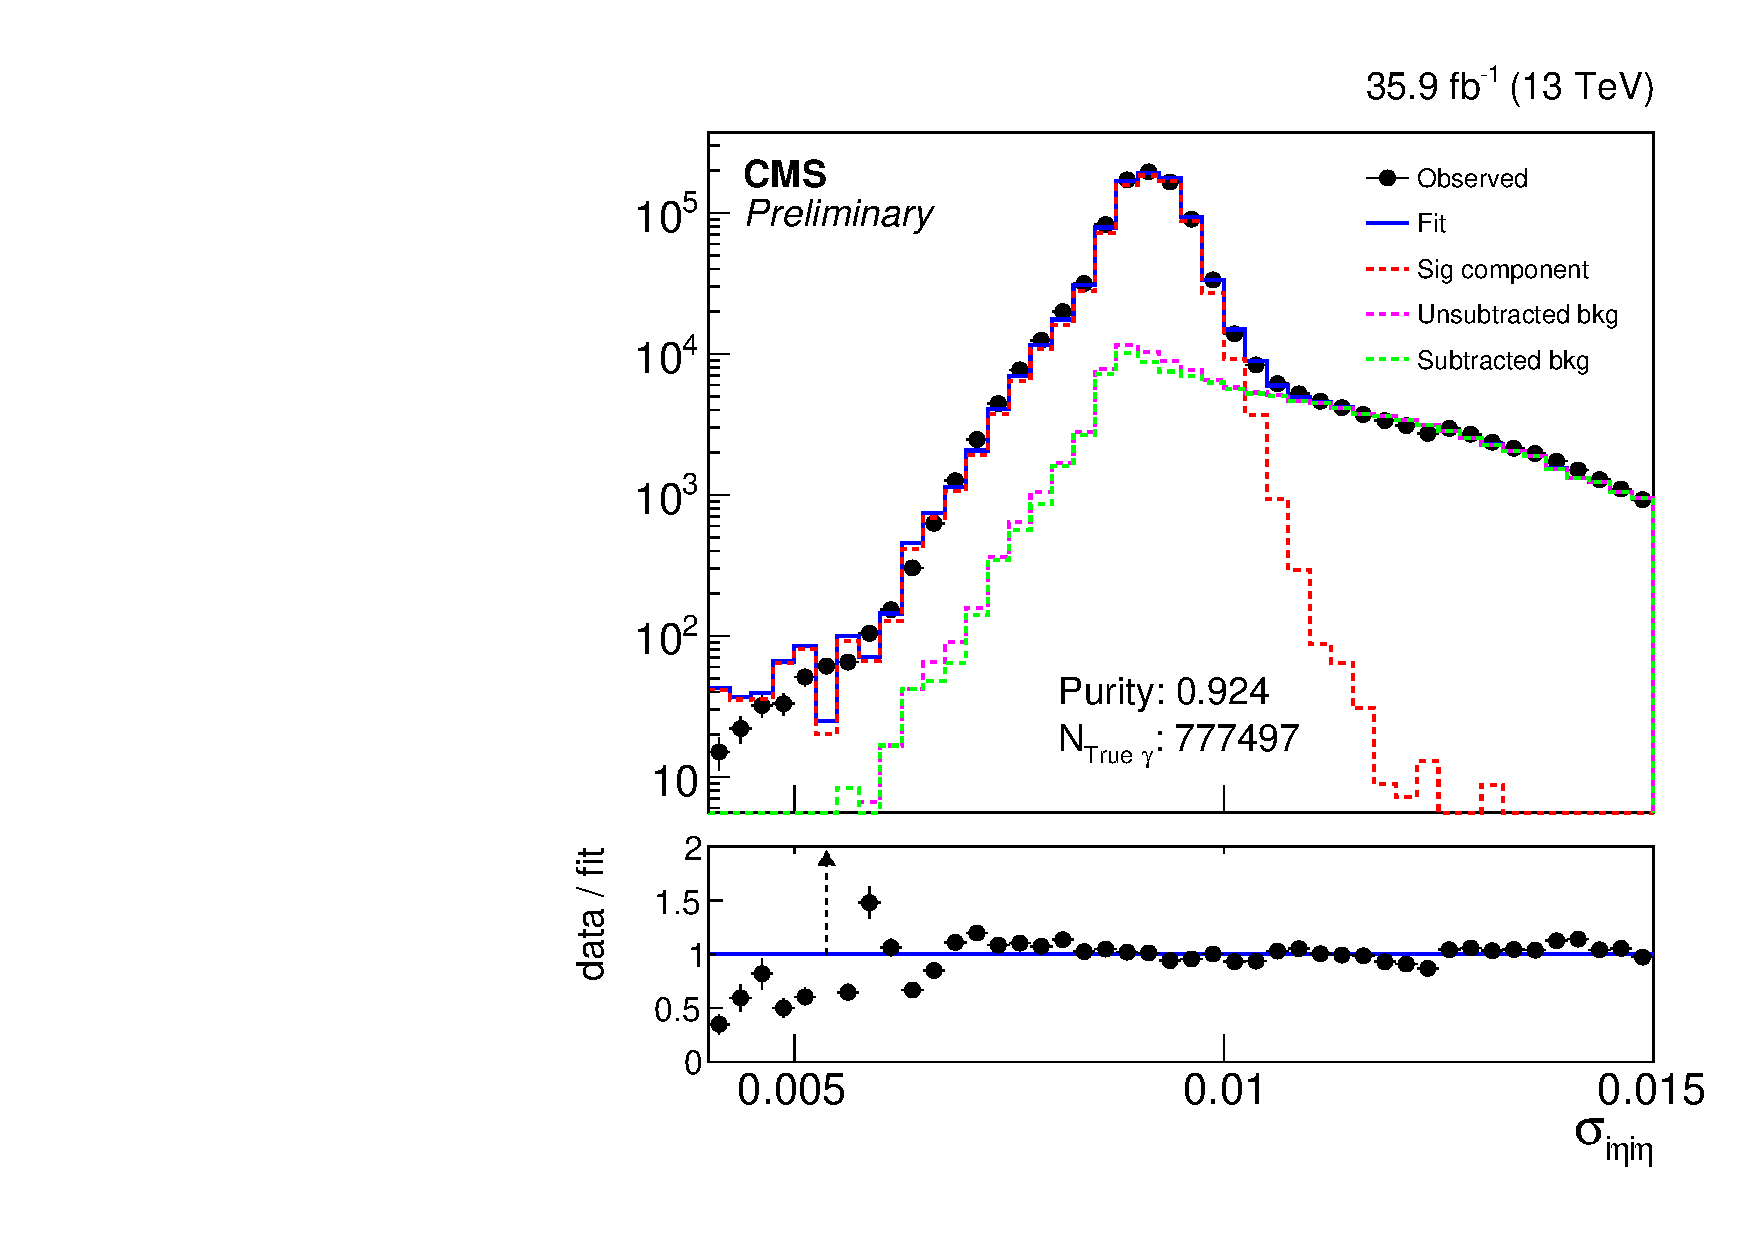
\includegraphics[width=0.45\textwidth]{Calibration/Figures/pvsf/ssfit_175_medium_far_logy.pdf}
  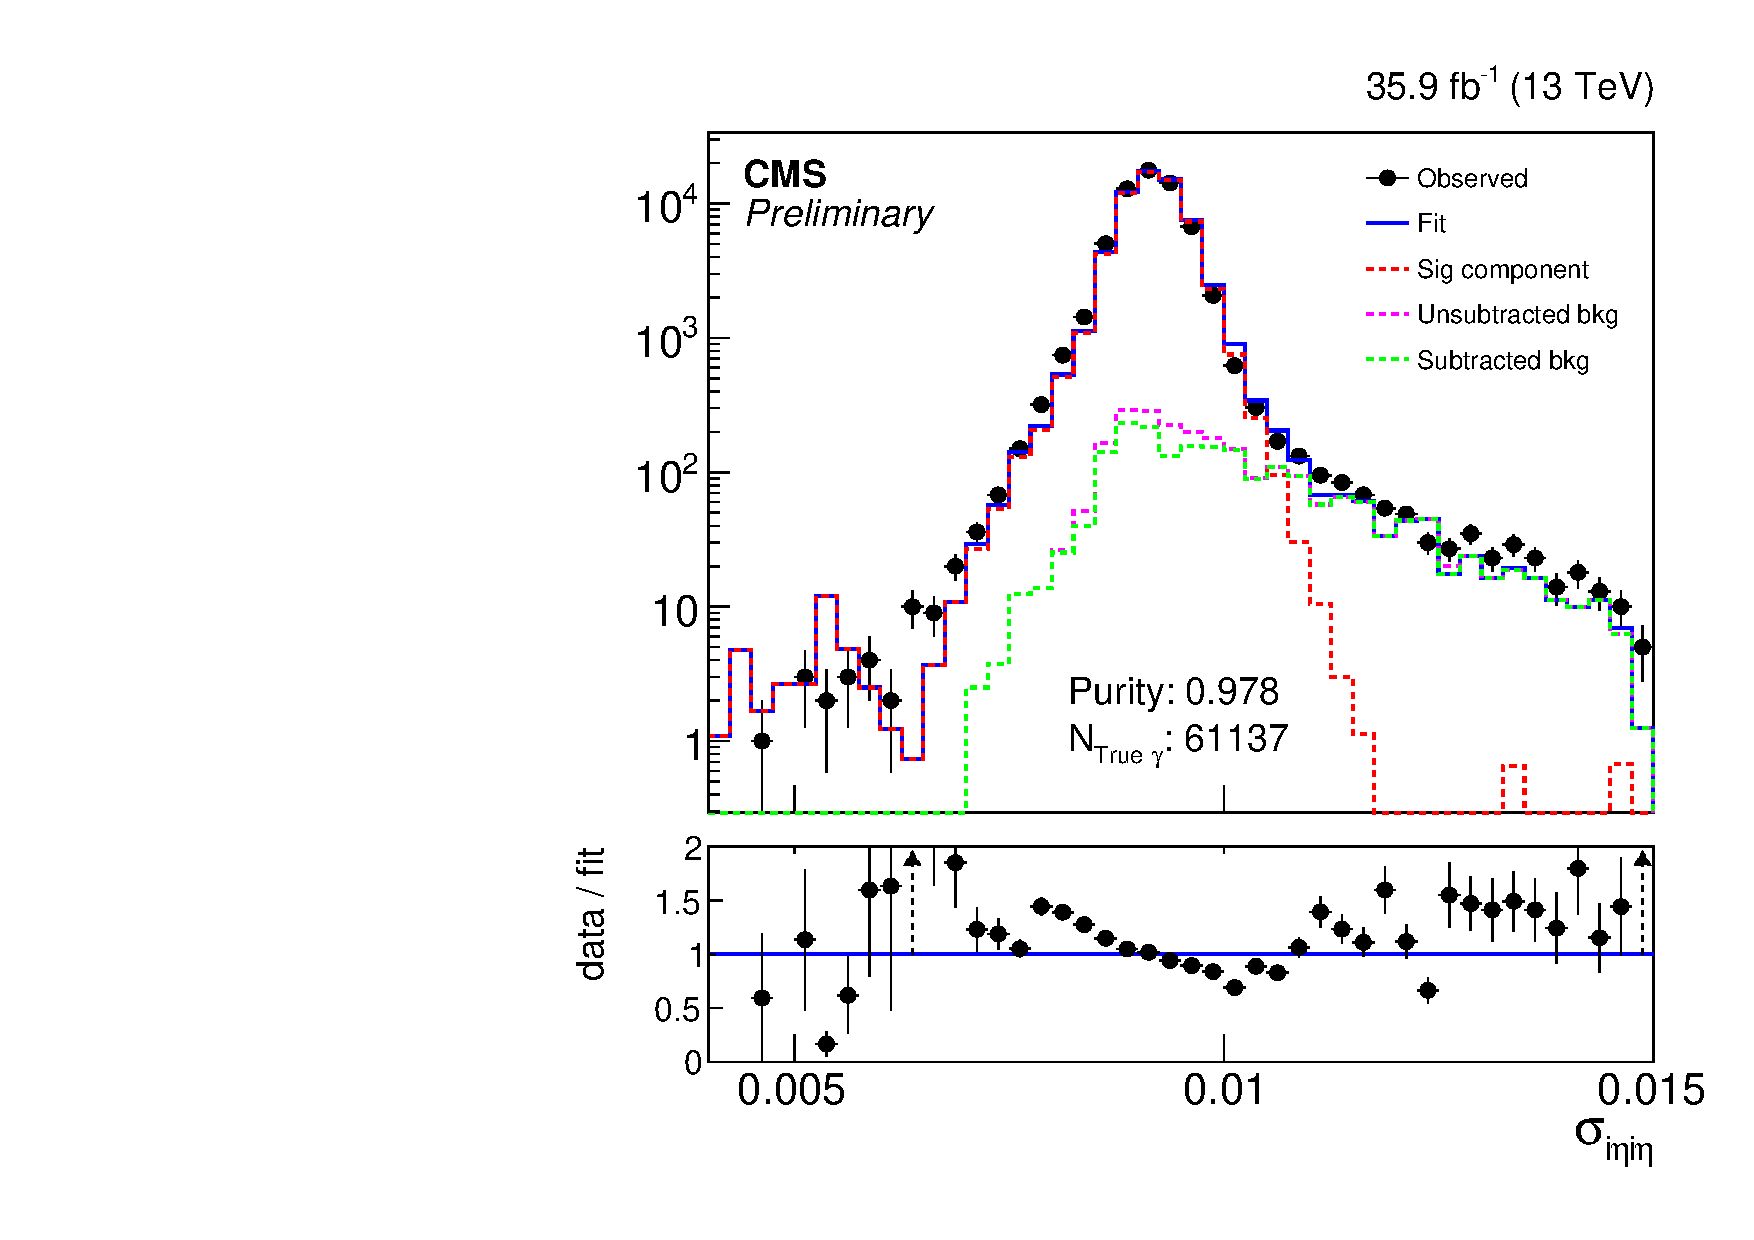
\includegraphics[width=0.45\textwidth]{Calibration/Figures/pvsf/ssfit_400_medium_far_logy.pdf}
  \caption{
    Fits to the \sieie\ distributions for the [175, 200] (left) and [400,$\infty$) (right) \pt\ bins using the [3.5,5.0] (top), [5.0,7.5] (middle), and [7.5,9.0] (bottom) isolation sidebands.
      The blue solid line represents the full fit model, the red dashed line its signal component, and the green dashed line its background component.
    }
  \label{fig:impurity-sideband}
\end{figure}

To measure the uncertainty due to the \ICH\ shape, we look at the \ICH\ for electrons in
\Zee\ events in both data and MC. 
Using these distributions, we obtain a data/MC scale factor which we apply to the MC true photon \ICH\ distribution to obtain a scaled MC distribution. 
This process is shown in Figure~\ref{fig:impurity-chiso}. 
Then, we recount the photons using this new distribution and take the difference in the values obtained using the raw MC and scaled MC distributions as a systematic uncertainty.

\begin{figure}[htbp]
  \centering
  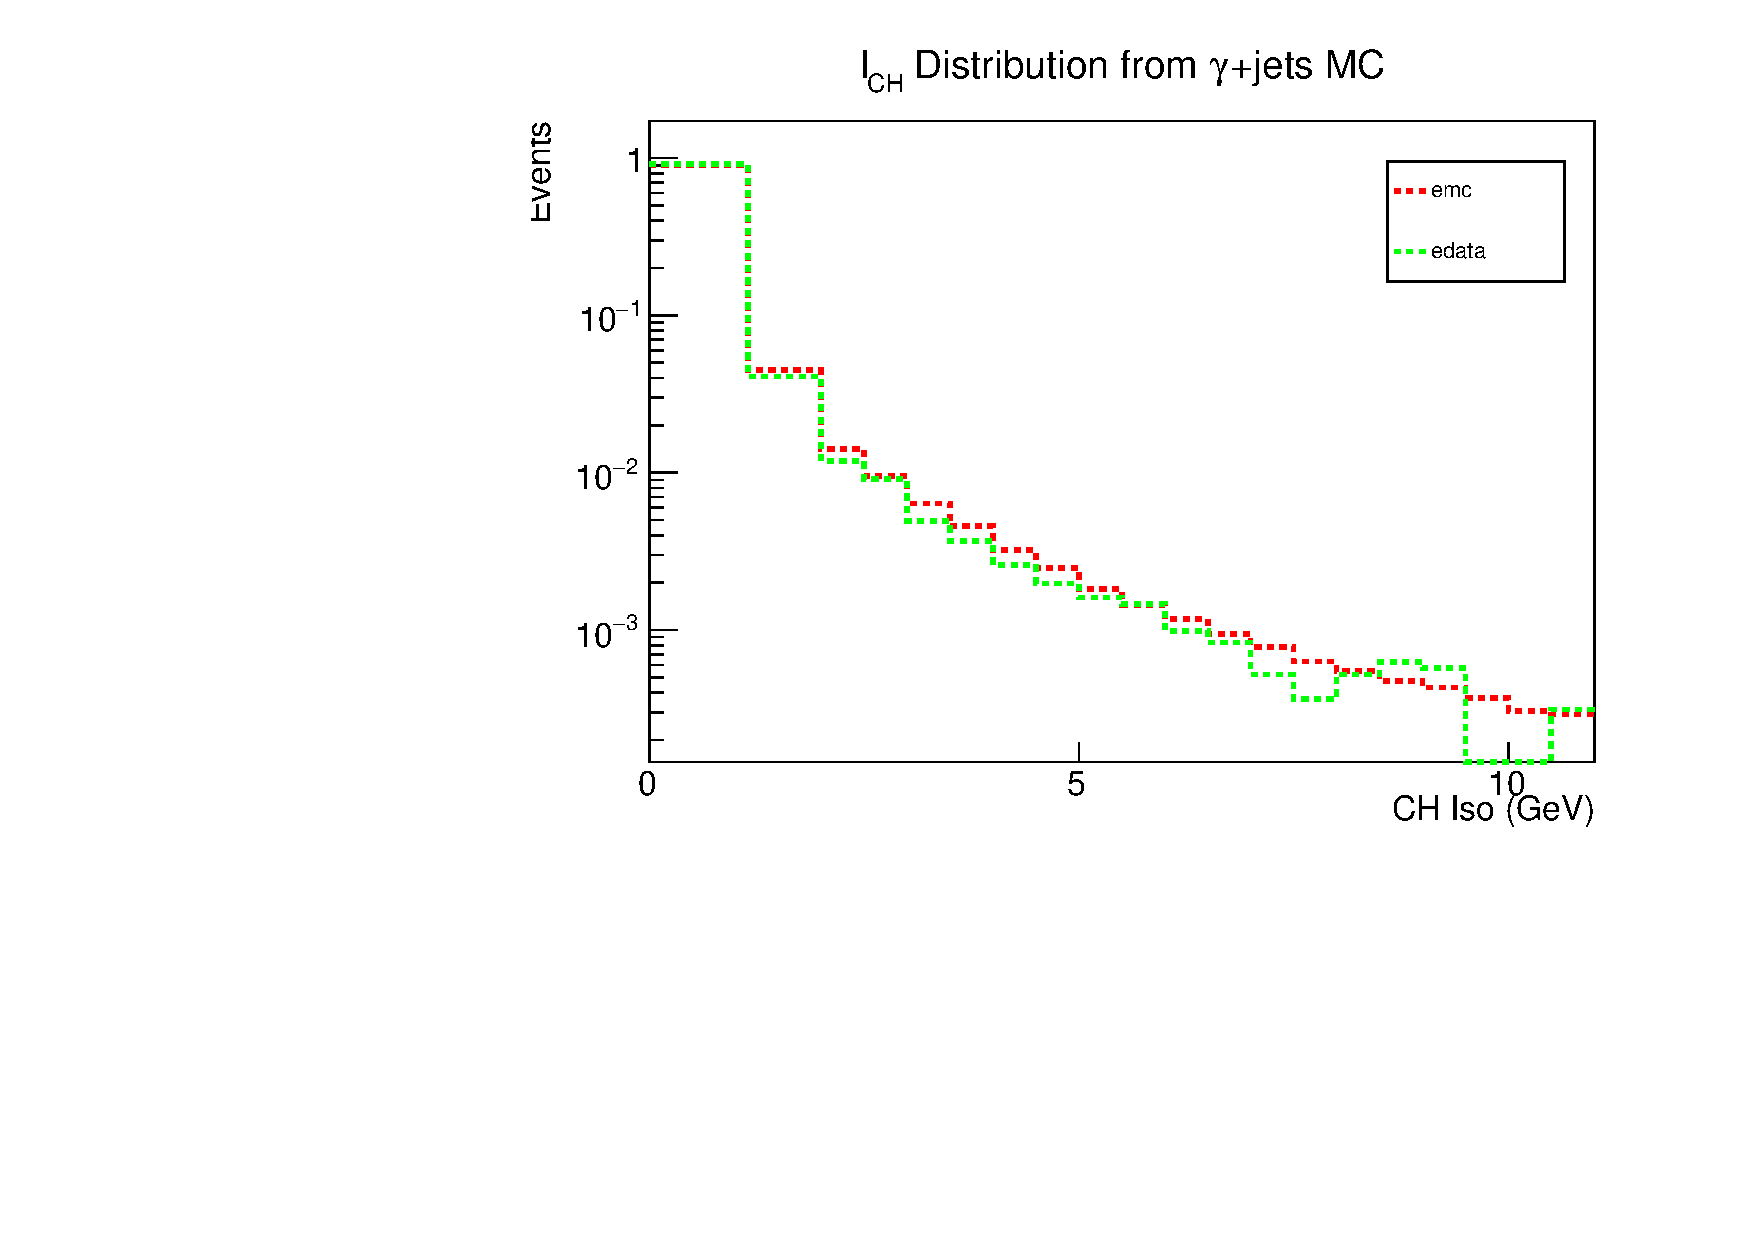
\includegraphics[width=0.45\textwidth]{Calibration/Figures/pvsf/chiso_electrons_logy.pdf}
  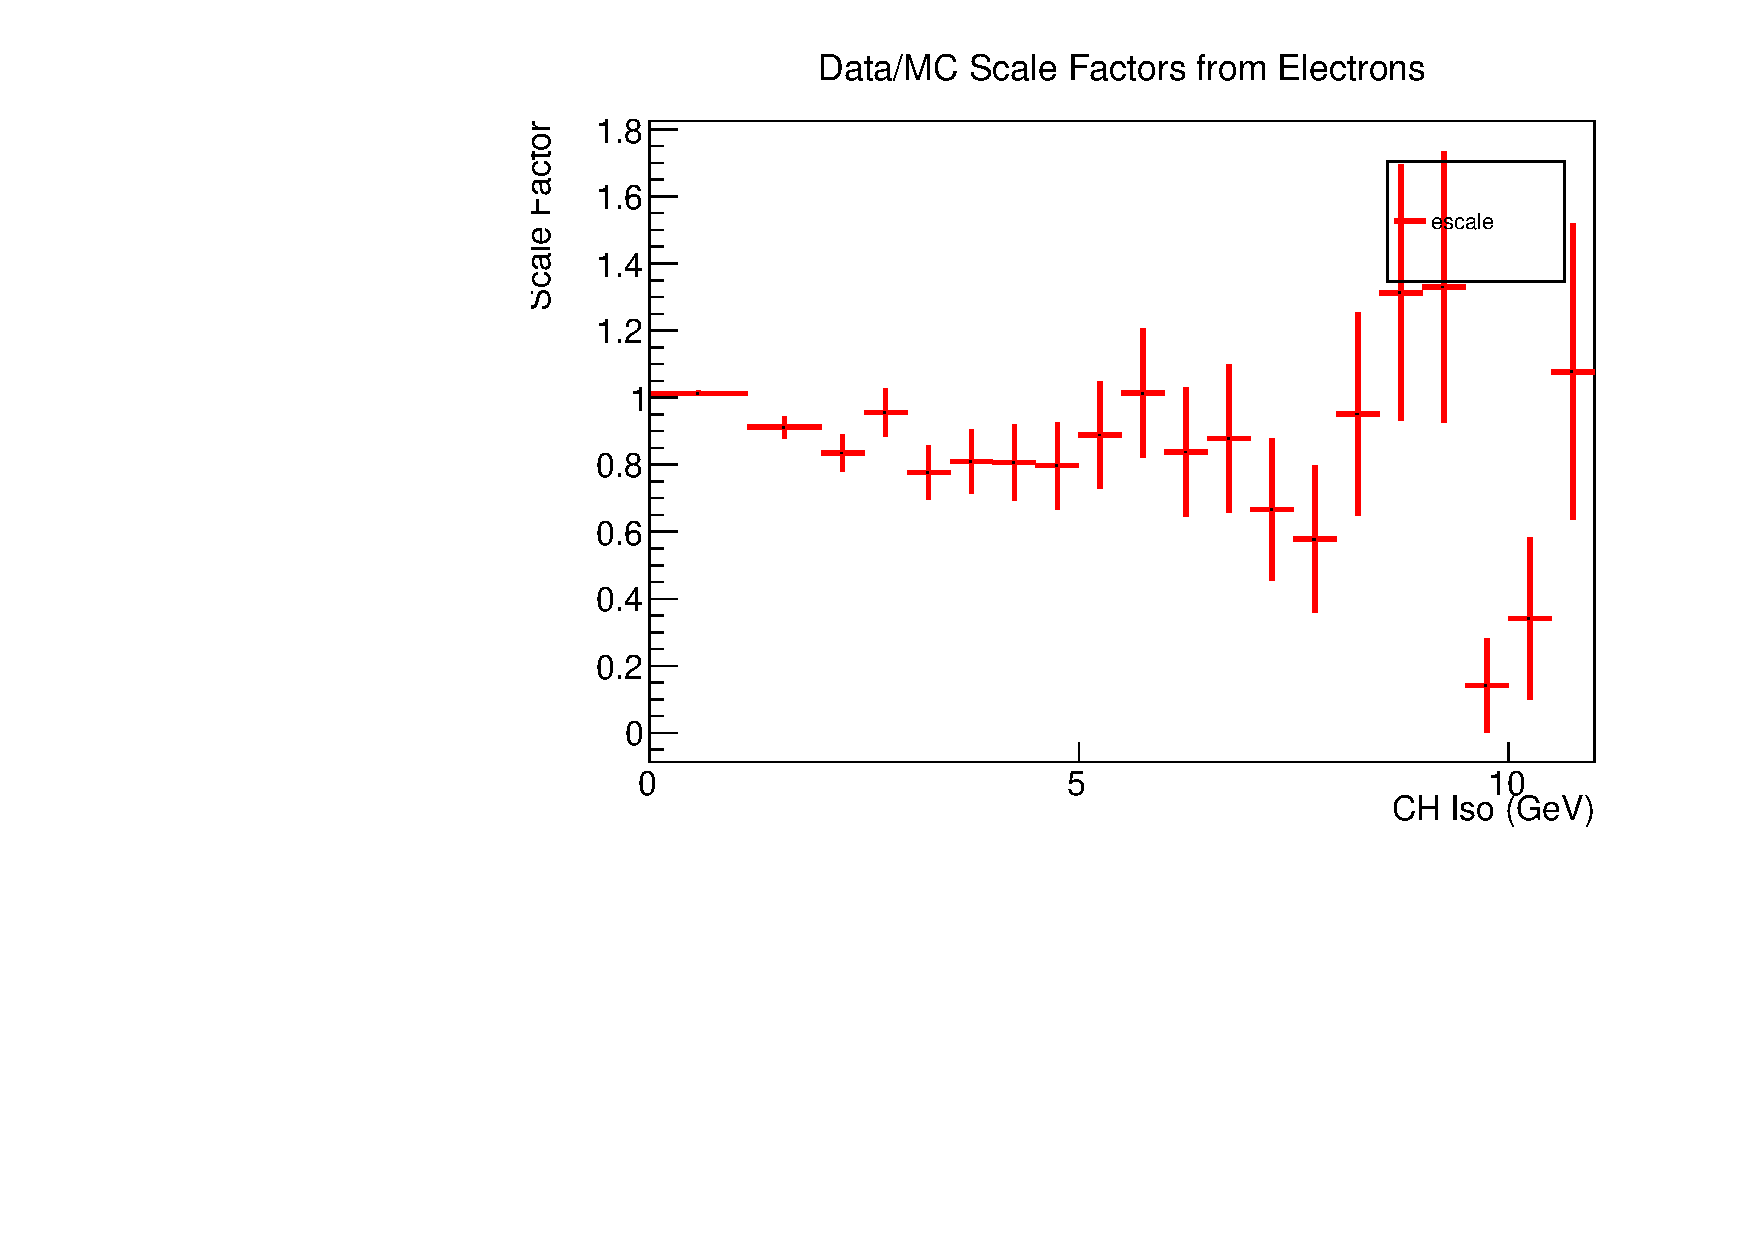
\includegraphics[width=0.45\textwidth]{Calibration/Figures/pvsf/chiso_scale.pdf}
  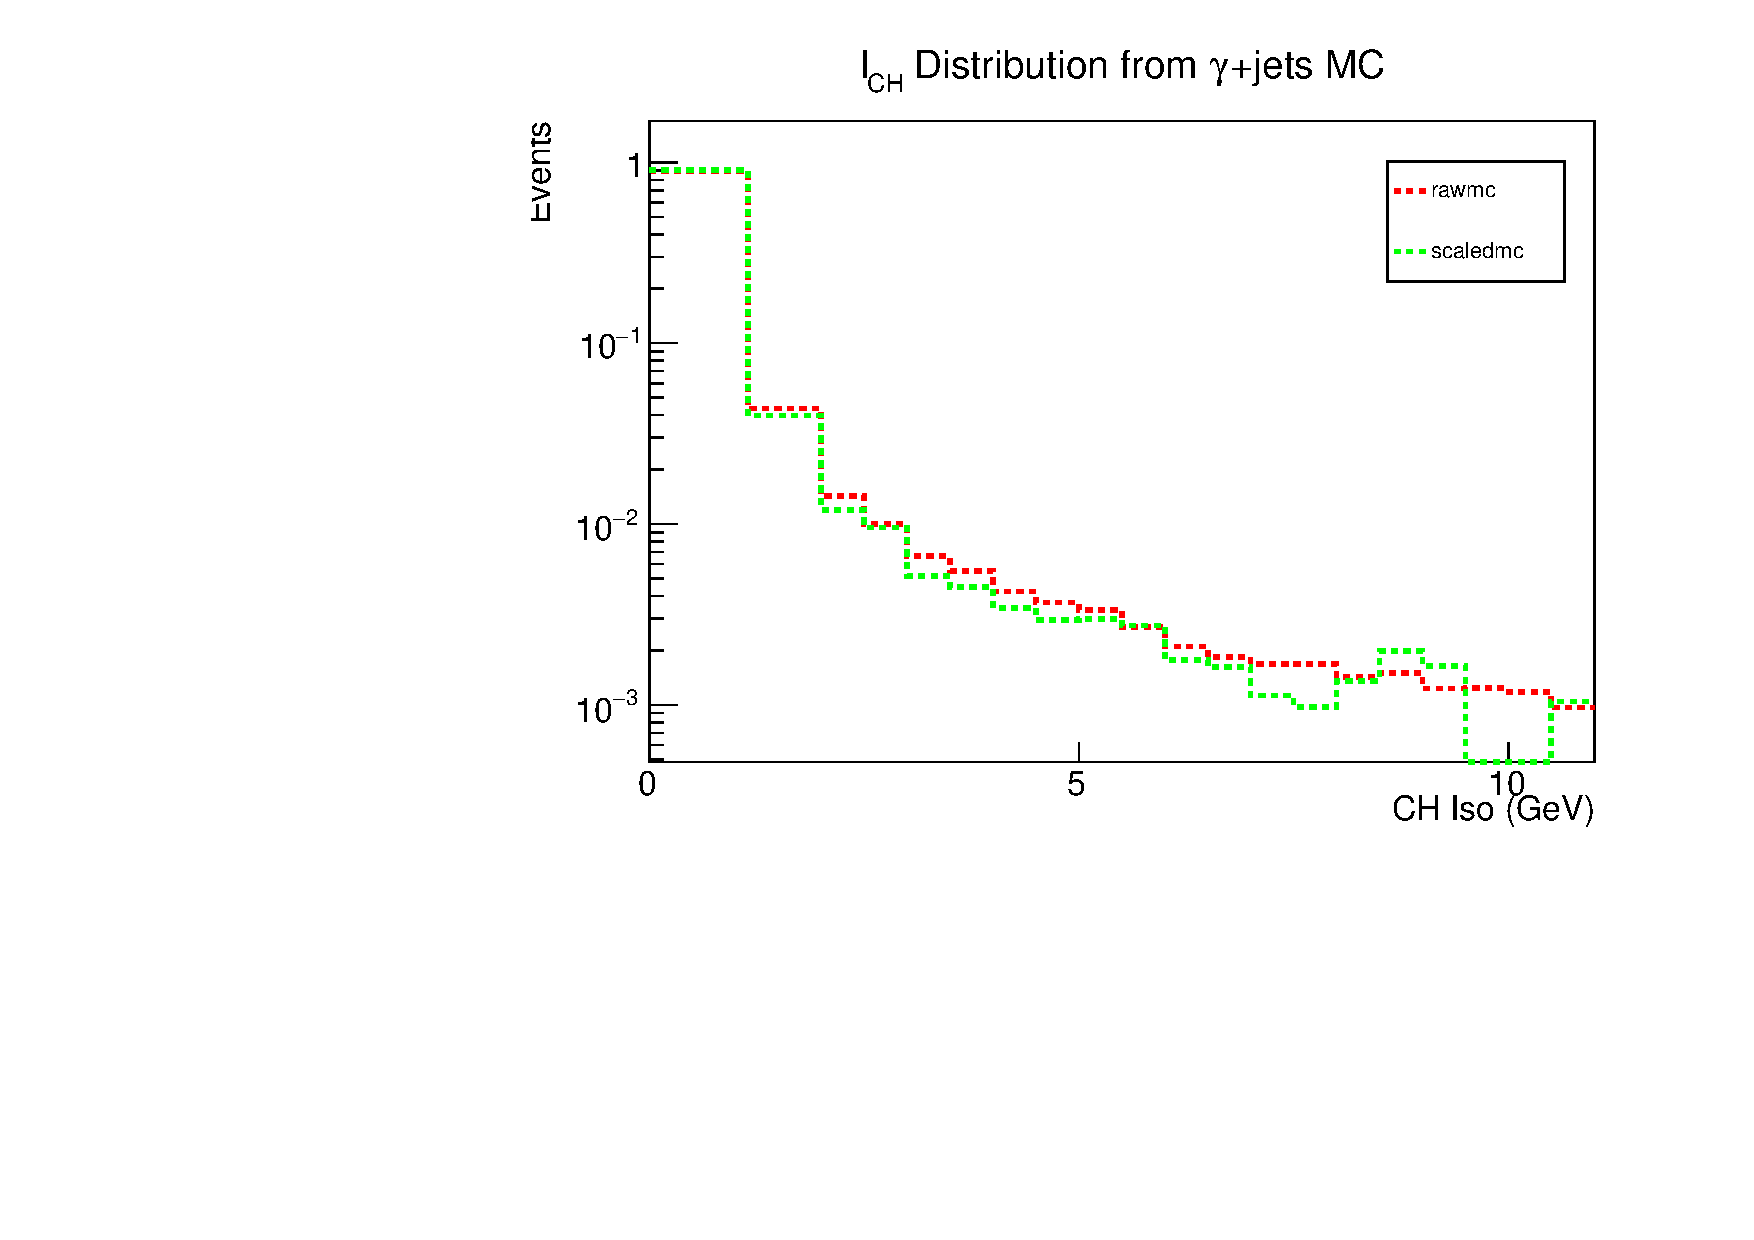
\includegraphics[width=0.45\textwidth]{Calibration/Figures/pvsf/chiso_photons_logy.pdf}
  \caption{
    Top left: \ICH\ distributions of electrons in data and MC in \Zee\ events.
    Top right: data/MC scale factor obtained from the electron \ICH\ distributions.
    Bottom: \ICH\ distributions of the MC photon objects used to estimate the amount of photon contamination in the background
    template, before and after applying the data/MC scale factor.
  }
  \label{fig:impurity-chiso}
\end{figure}

To measure the uncertainty due to the signal template \sieie\ shape, we look at the \sieie\ distributions for electrons in both data and MC. Again we compare \Zee\ events in data and MC.
From the \sieie\ distributions of high-purity electron samples, obtain a data/MC scale factor which we apply to the MC true photon \sieie\ distribution to obtain a scaled MC distribution.
Then, we recount the photons using this new distribution and take the difference in the values obtained using the raw MC and scaled MC distributions as a systematic uncertainty. 
The difference between fits with and without the \sieie\ scaling are shown in Figure~\ref{fig:impurity-sieie}.

\begin{figure}[htbp]
  \centering
  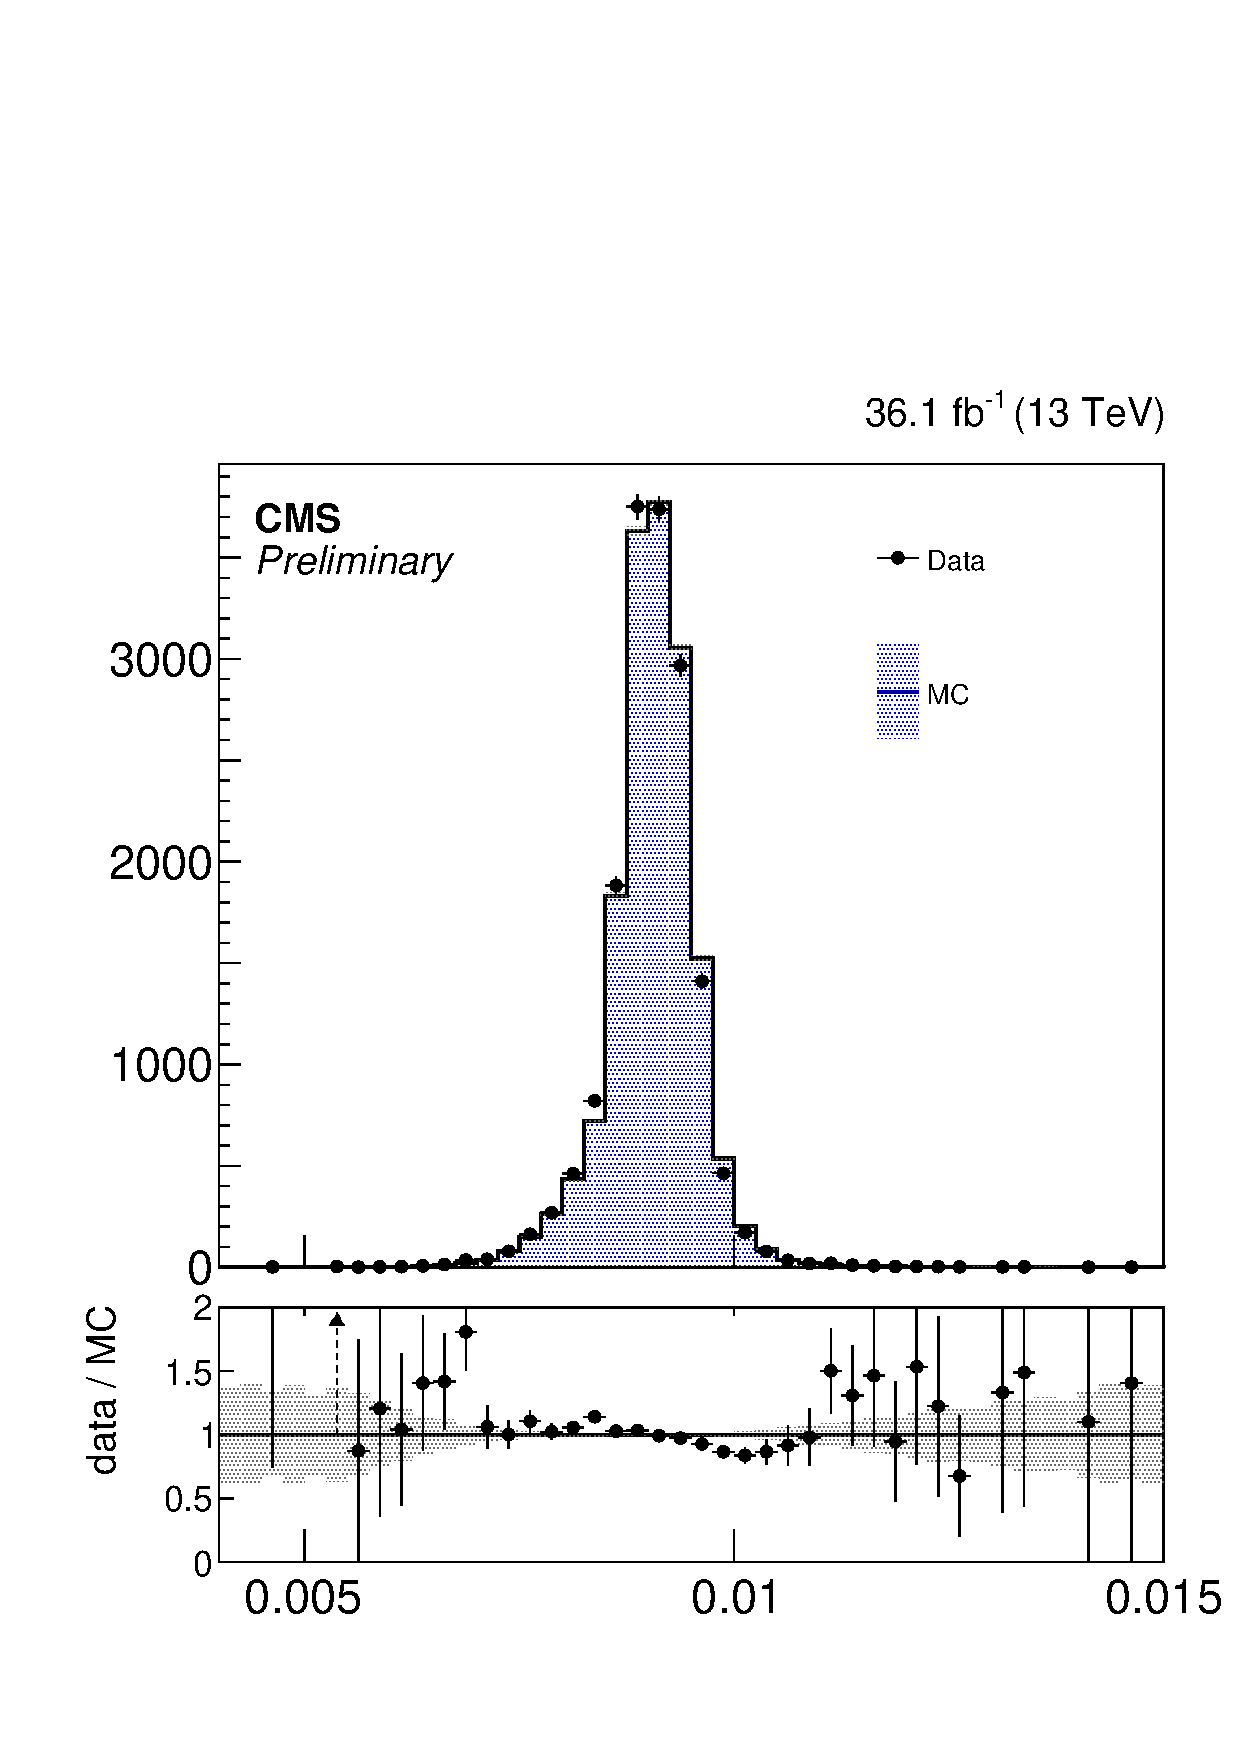
\includegraphics[width=0.45\textwidth]{Calibration/Figures/pvsf/sieie_ratio.pdf}
  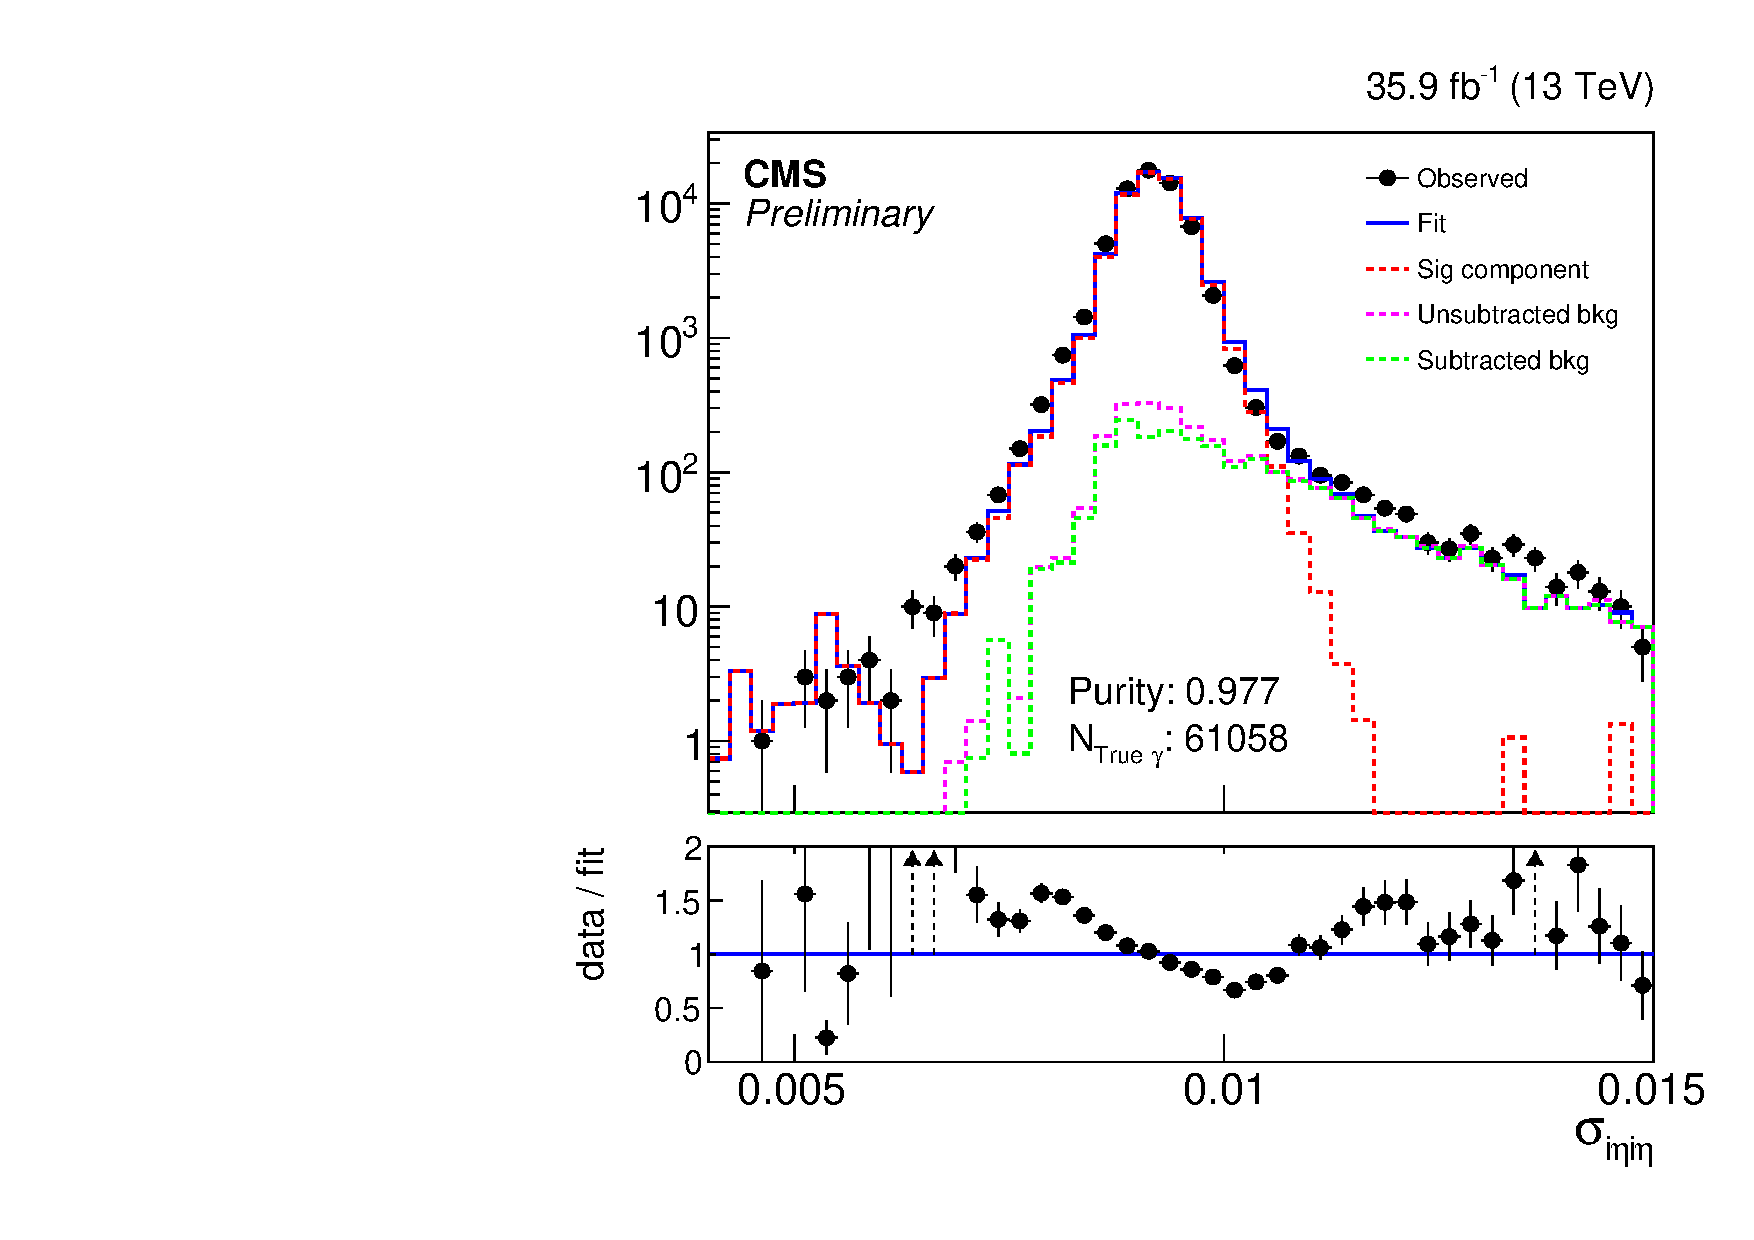
\includegraphics[width=0.45\textwidth]{Calibration/Figures/pvsf/ssfit_400_medium_shape_logy.pdf}
  \caption{
    Left: Comparison of \sieie\ distributions between data and MC in \Zee\ events. 
    Lower panel shows the data/MC \sieie\ scale factor.
    Right: Result of the fit with true-photon template with the data/MC \sieie\ scale factor applied to the true-photon template.
  }
  \label{fig:impurity-sieie}
\end{figure}

To estimate the uncertainty due to statistical fluctuations in our background templates, we generate toys from the background template from data. 
We then repeat the fit with each of these toys and plot the distribution of the difference between the purity value obtained from the toy templates versus the nominal template. 
We take the standard deviation of this distribution, shown in Figure~\ref{fig:impurity-toys}, as a systematic uncertainty.

\begin{figure}[htbp]
  \centering
  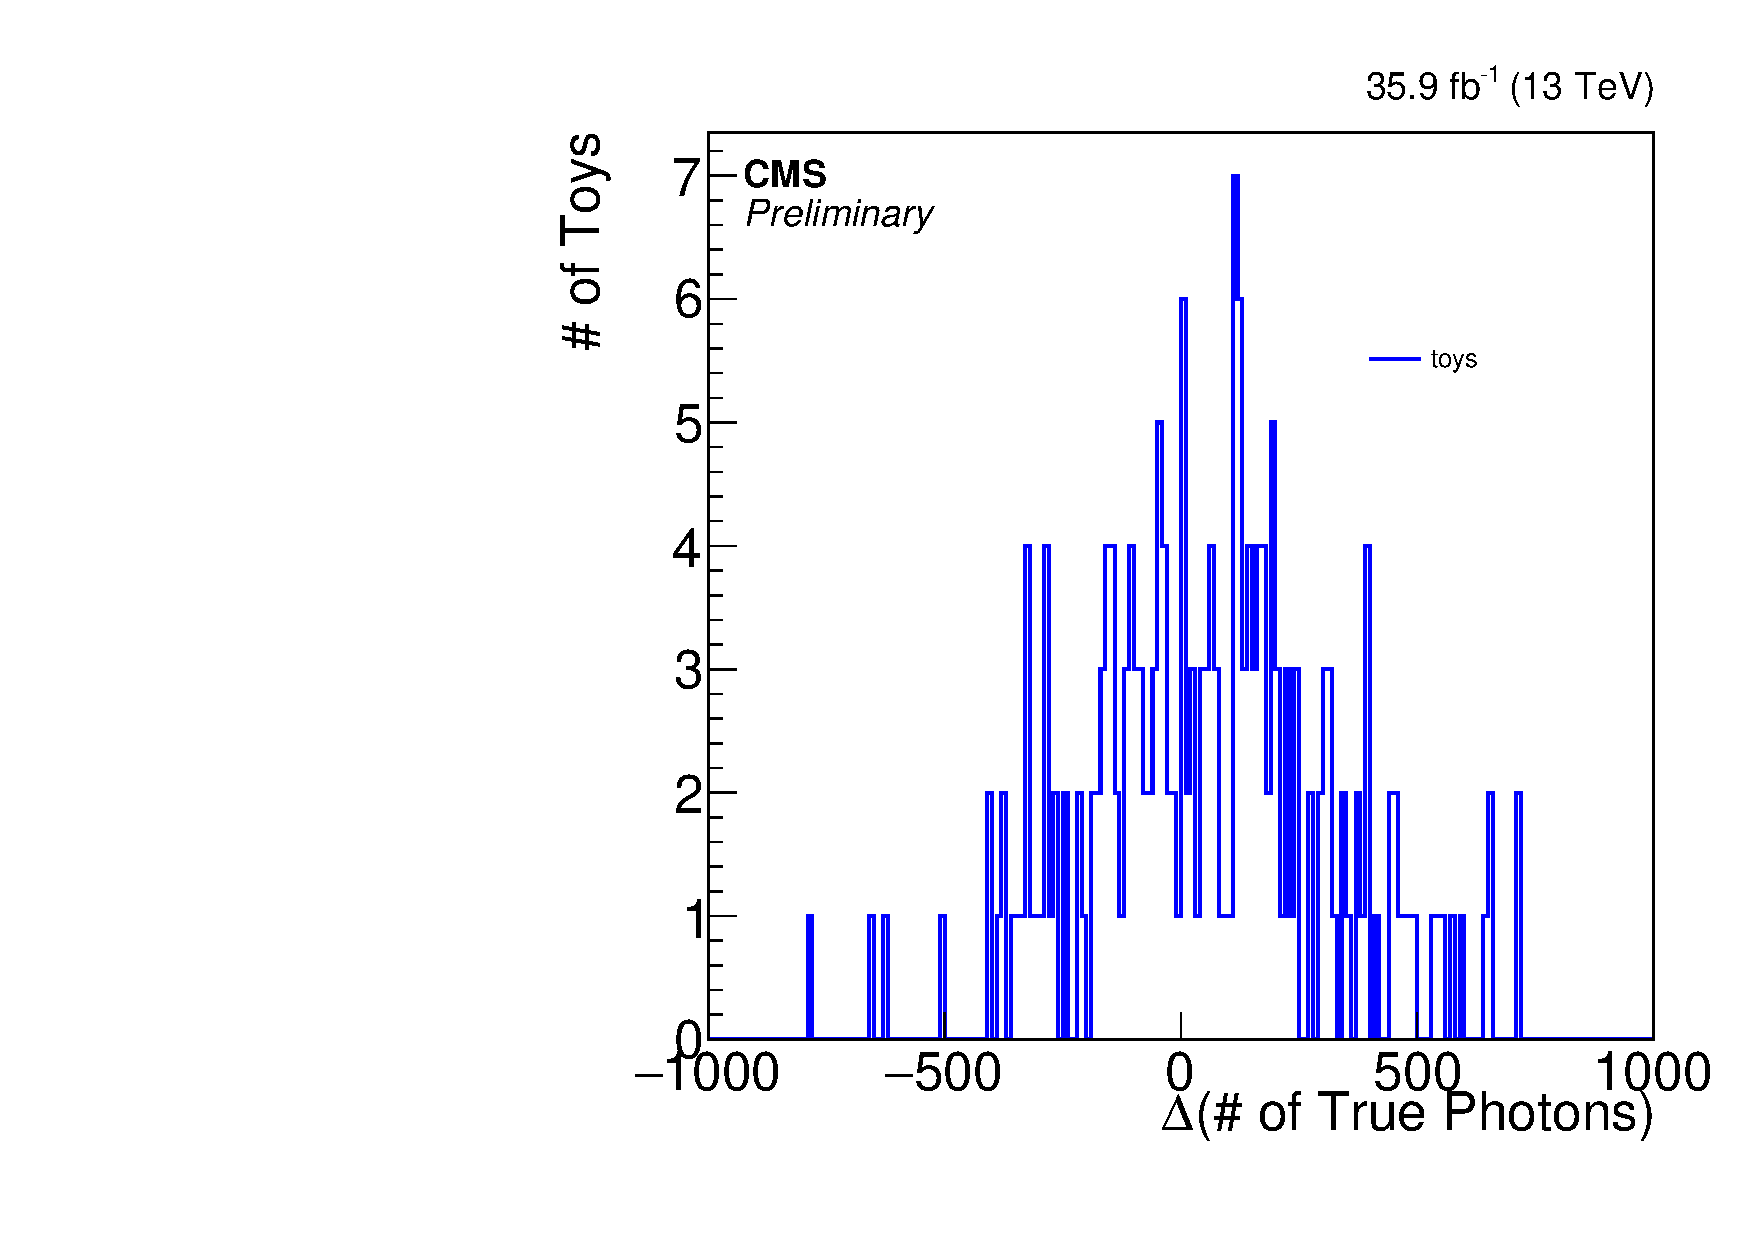
\includegraphics[width=0.45\textwidth]{Calibration/Figures/pvsf/ssfit_175_medium-pixel-monoph_toyyield_dist.pdf}
  \caption{
    Shift in true-photon yields, extracted from alternative fits varying the background template within its statistical uncertainty. 
    Nominal photon count in this specific \ETg\ bin is $6.64\times 10^{5}$.
  }
  \label{fig:impurity-toys}
\end{figure}

The values obtained for each systematic uncertainty on the true photon count of the denominator are shown in Table~\ref{tab:impurity-systs} in bins of \pt. 
The relative uncertainties on the numerator are similar, and in the efficiency, each uncertainty source is considered as fully correlated.

\begin{table}[htbp]
  \begin{center}
    \caption{Relative uncertainties on the estimated number of true photons in the denominator sample.}
    \label{tab:impurity-systs}
    \begin{tabular}{ |c|c c c c| }
    \hline
    \pt\ Range & \multicolumn{4}{ |c| }{Sources of Systematic Uncertainty} \\
     (GeV) & Sideband & \ICH\ Shape & Signal Shape & Bgkd. Stats \\
    \hline
     (175, 200)  & 0.09 & 0.18 & 0.05 & 0.04 \\
     (200, 250)  & 0.01 & 0.16 & 0.06 & 0.03 \\
     (250, 300)  & 0.14 & 0.16 & 0.06 & 0.05 \\
     (300, 350)  & 0.12 & 0.16 & 0.07 & 0.08 \\
     (350, 400)  & 0.23 & 0.11 & 0.05 & 0.10 \\
     (400, $\infty$)  & 0.27 & 0.09 & 0.05 & 0.05 \\
    \hline
    \end{tabular}
  \end{center}
\end{table}

The MC effiiency of the \Pgg-specific ID is determined by counting the number of truth-matched photons passing \egamma\ part of the ID and the full ID. 
However, there is a complication, the \gj\ region in data has approximately 5\% contamination from electrons before applying the pixel veto, as shown in Figure~\ref{fig:pvsf_contam}. 
Thus, we combine appropriately cross-section weighted \gj, \wj, and \ttbar\ samples and truth match to both electrons and photons. 
Additionally, we apply a 14\% uncertainty on the \wj\ and \ttbar\ yields to account for the NLO cross-section ratio uncertainties with respect to \gj\ at this \pt\ range that is uncorrelated between the numerator and denominator as a negligible amount of electron events survive the pixel veto.

\begin{figure}[htbp]
  \begin{center}
    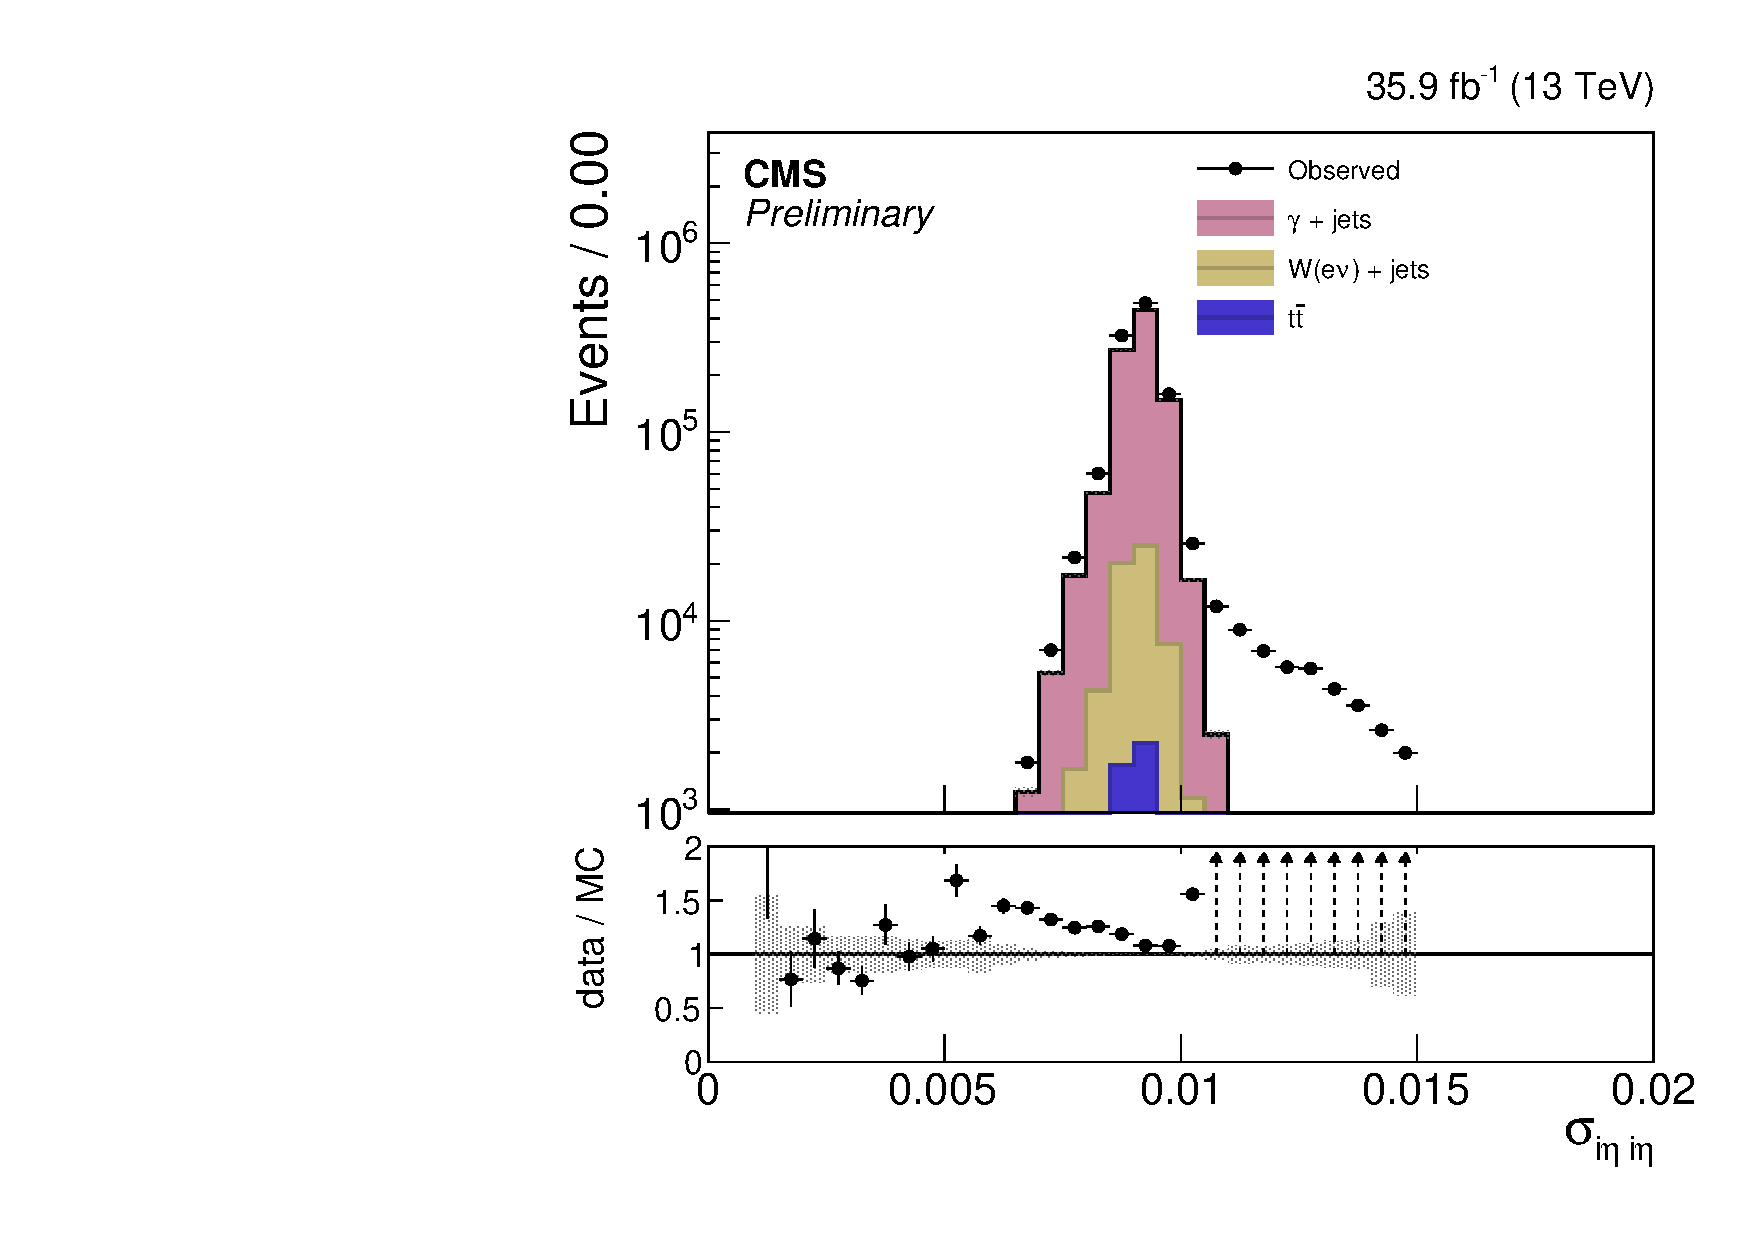
\includegraphics[width=0.48\textwidth]{Calibration/Figures/pvsf/gjets_sieie.pdf}
    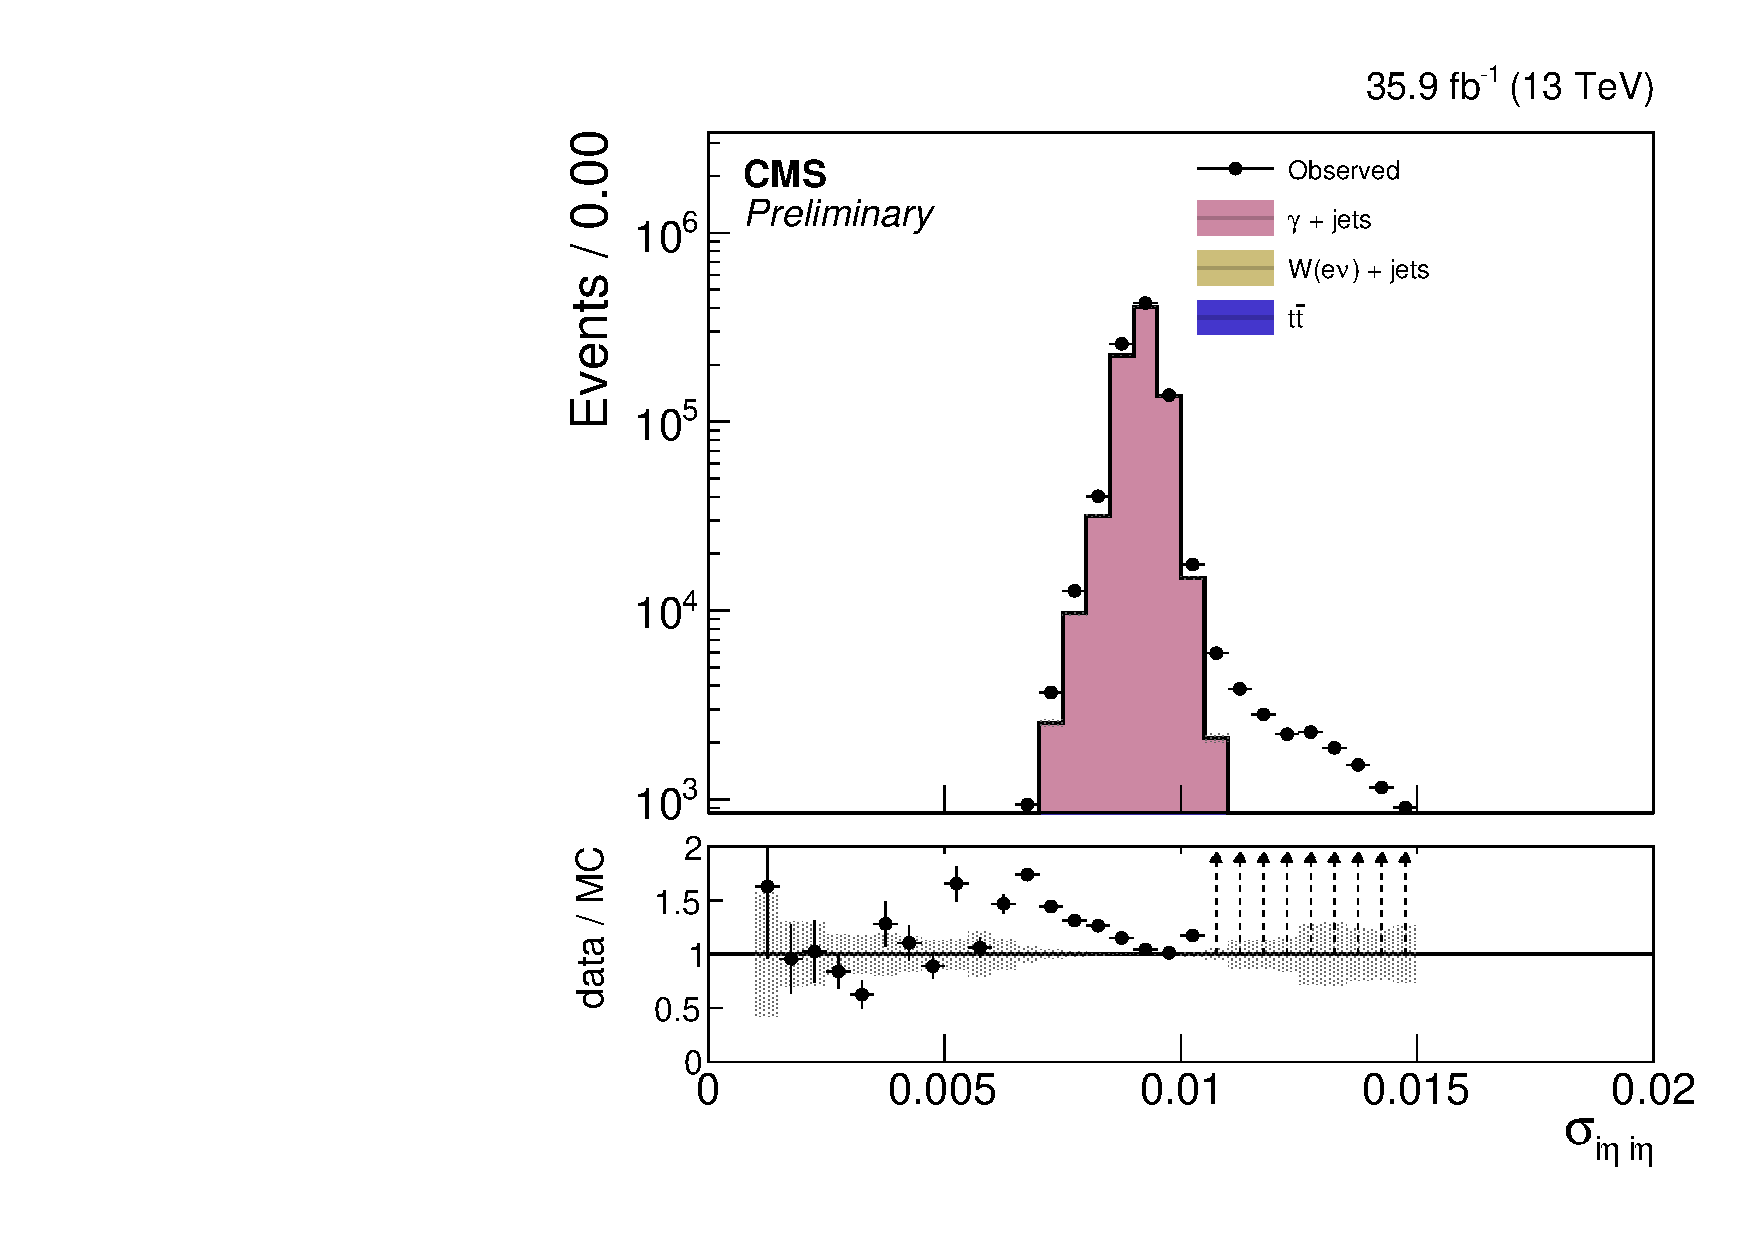
\includegraphics[width=0.48\textwidth]{Calibration/Figures/pvsf/gjets_sieiePixelVeto.pdf}
    \caption{
      Electron contamination in \gj\ region before (left) and after (right) applying the pixel seed veto.
    }
    \label{fig:pvsf_contam}
  \end{center}
\end{figure}
 
The data efficiency, MC efficiency, and the scale factor for the \Pgg-specific ID as a function of \pt\ are shown in Figure~\ref{fig:pvsf_results}. 
As there is no significant trend in the scale factor as a function of \pt\, we apply a flat scale factor of $0.984 \pm 0.009$ for all of the MC-based background and signal models in the analysis.

\begin{figure}[htbp]
  \begin{center}
    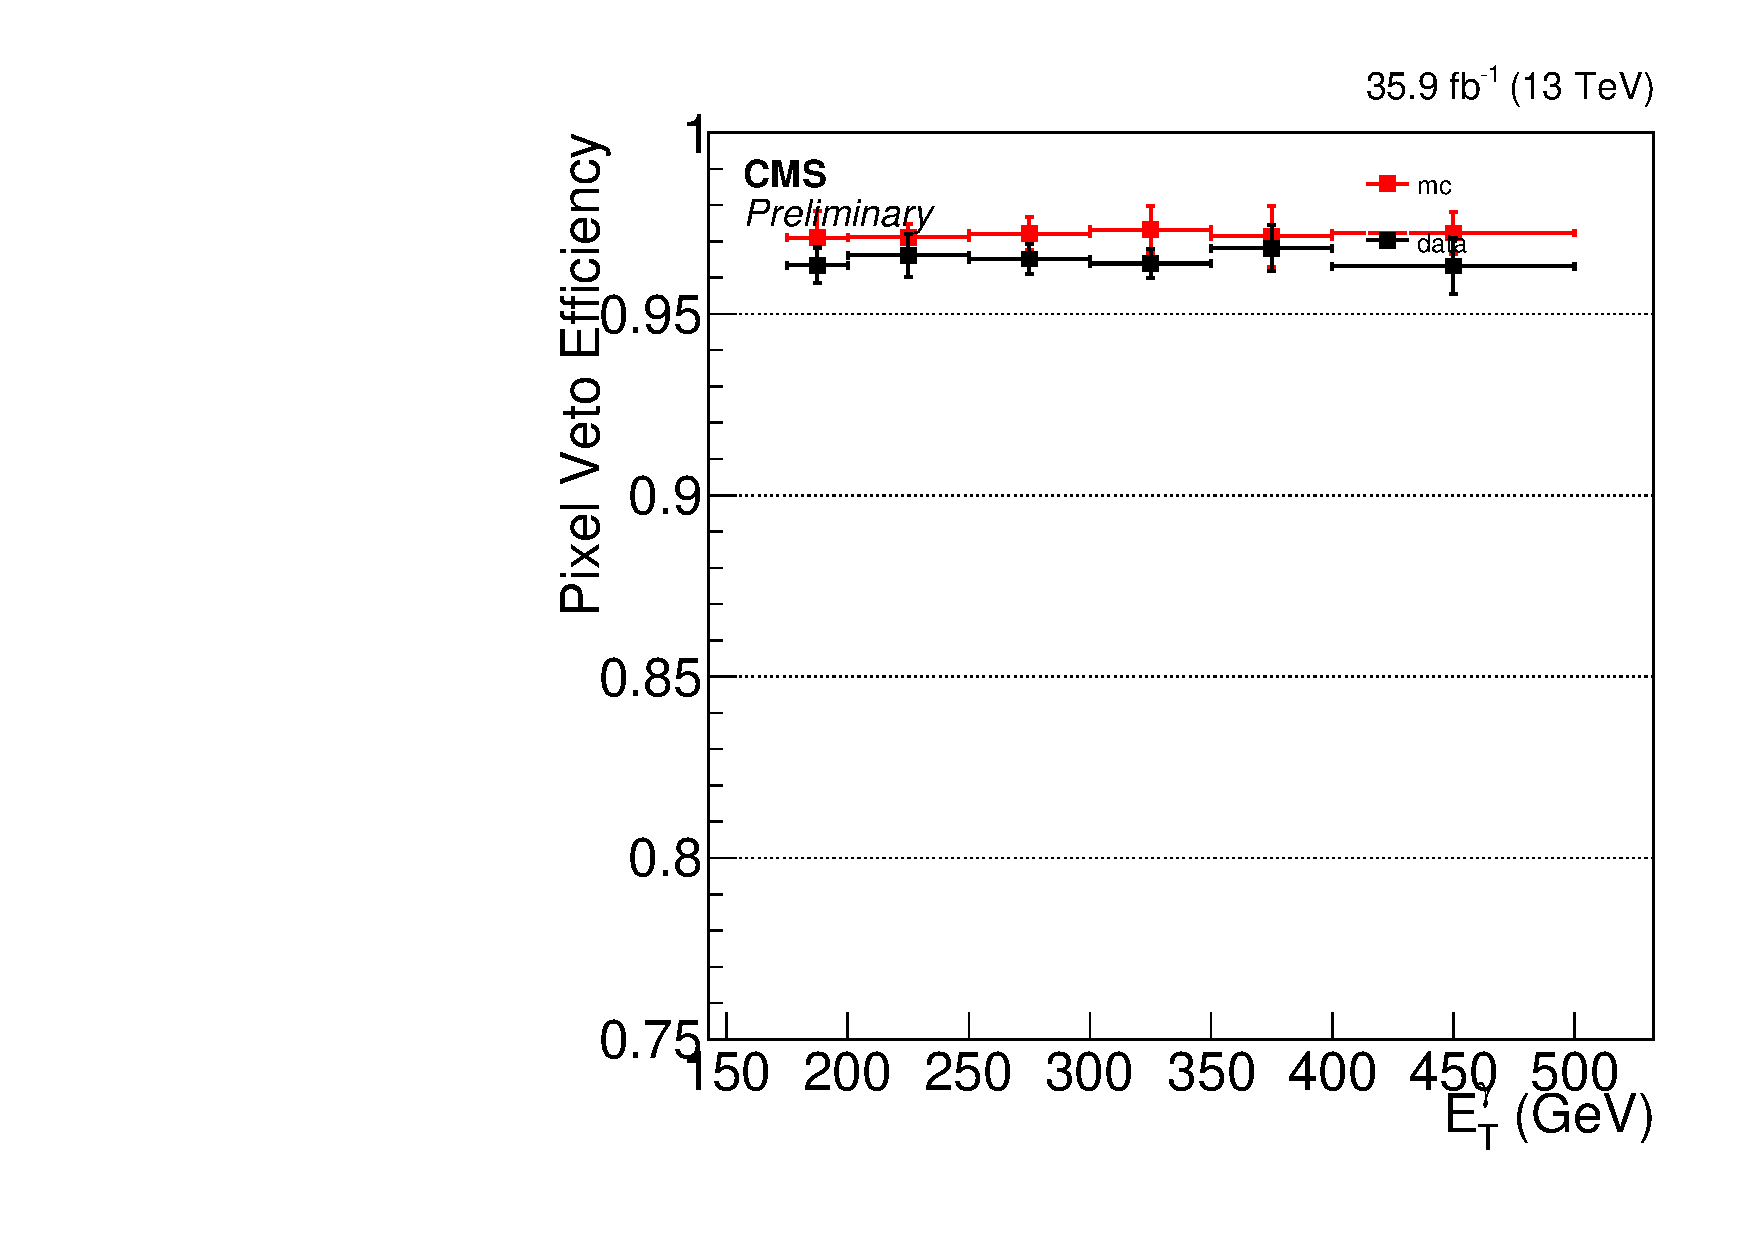
\includegraphics[width=0.48\textwidth]{Calibration/Figures/pvsf/efficiency_barrel_medium.pdf}
    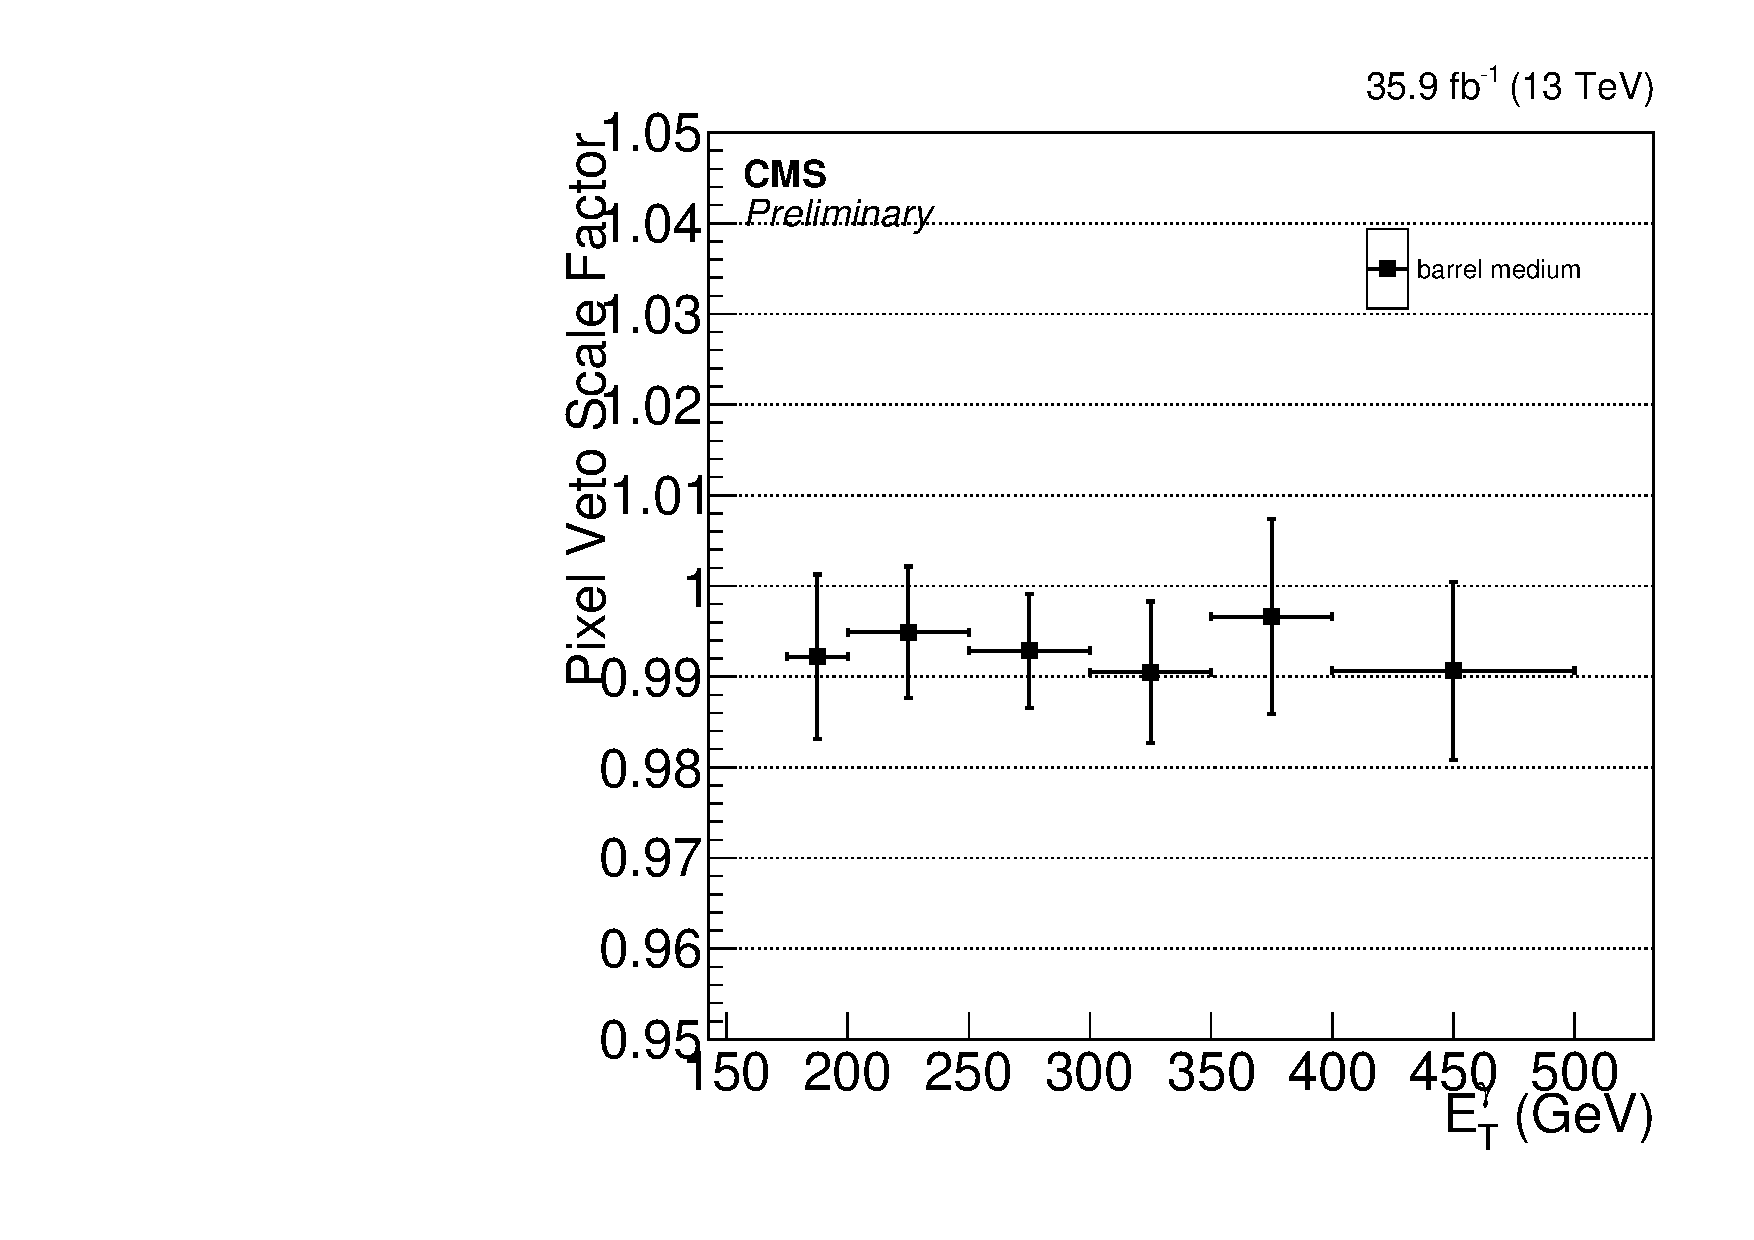
\includegraphics[width=0.48\textwidth]{Calibration/Figures/pvsf/scalefactor_barrel_medium.pdf}
    \caption{
      Photon pixel veto efficiencies (left) and correspending scale factor (right) as a function of photon \pt.
    }
    \label{fig:pvsf_results}
  \end{center}
\end{figure}

\section{Lepton Scale Factors}

\section{Jet Energy Scale}
